\documentclass[a4paper,11pt,twoside,openright]{book} % Type du document

% compiler avec : pdflatex, bibtex, pdflatex, pdflatex


% +---------------------------------------------------------------+
% | Language
% +---------------------------------------------------------------+
\usepackage[T1]{fontenc}
\usepackage[utf8]{inputenc}
\usepackage[french]{babel}
\usepackage{pdfpages}


\usepackage[acronym, toc]{glossaries}

\makeglossaries

\newglossaryentry{GNOME}
{
	name=gnome,
	description={Environnement graphique pour plateformes GNU/LINUX}
}


\newglossaryentry{filesystem}
{
	name=filesystem,
	description={Organisation hiérarchique des fichiers au sein d'un système d'exploitation.}
}

\newglossaryentry{bloatwares}
{
	name=bloatwares,
	description={Ensemble de logiciels superflus pour une OS}
}


\newglossaryentry{API}
{
	name=api,
	description={Application Programming Interface -> ensemble normalisé de classes, de méthodes, de fonctions et de constants qui sert de façade par laquelle un logiciel offre des services à d'autres logiciels.}
}

\newglossaryentry{Operating System}
{
	name=os,
	description={Ensemble de programmes qui dirige l'utilisation des ressources d'un ordinateur par des logiciels applicatifs.}
}


\newacronym{lts}{LTS}{Long Term Support}
\newacronym{gui}{GUI}{Graphical user interface}
\newacronym{os}{OS}{Operating System}
\newacronym{de}{DE}{Desktop Environment}
\newacronym{acl}{ACL}{Access Control List}
\newacronym{vnc}{VNC}{Virtual Network Computing}

\newif\ifisconfidential	\isconfidentialfalse

\newif\ifisdraft\isdraftfalse



% +---------------------------------------------------------------+
% | Paramètres
% +---------------------------------------------------------------+

\newcommand{\TBtitle}{Sécurisation de logiciels et distribution Linux}
% \newcommand{\TBsubtitle}{Sous-titre}%laisser vide si pas de sous-titre
\newcommand{\TByear}{2020}
\newcommand{\TBacademicYears}{2019-2020}

\newcommand{\TBdpt}{Département des Technologie de l'information et de la communication (TIC)}
\newcommand{\TBfiliere}{Filière Télécommunications}
\newcommand{\TBorient}{Orientation Sécurité de l'information}

\newcommand{\TBauthor}{Jeremy Zerbib}
\newcommand{\TBsupervisor}{Prof. Daniel Rossier}
\newcommand{\TBindustryContact}{Prof. Daniel Rossier}
\newcommand{\TBindustryName}{REDS}
\newcommand{\TBindustryAddress}{%
  Route de Cheseaux 1\\
  CP 521\\
  1400 Yverdon-les-Bains
}

% Confidentiel?
% uncomment if confidential / comment if not confiential
% \isconfidentialtrue

\newcommand{\TBresumePubliable}{
Les études à l'\textit{HEIG-VD} sont sur le point de connaître un changement de programme assez drastique. 
En effet, un remaniement des sections, départements et programmes sont mis en place pour la rentrée scolaire de Septembre 2020.
L'introduction d'une formation en \textit{ingénierie des données} et les changements de programme des départements existants amènent à penser que l'introduction d'un système Linux.
C'est pourquoi une distribution sur mesure pour l'\textit{HEIG-VD} serait la bienvenue 
\newline 
De plus, l'école déplore que certaines conditions générales d'utilisation (\textit{CGU}) ne soient pas respectées. 
En effet, l'utilisation des logiciels fournis par l'école doit être faite dans le cadre scolaire sans pouvoir déborder sur une utilisation personnelle.
Ainsi, dans le cadre de ce travail, une plateforme portable, disponible sur Internet par exemple, sera mise à disposition des étudiants pour qu'il puisse travailler avec ces outils en toute légalité.

}

% +---------------------------------------------------------------+



% +-[set path]-------------------------------------+
\usepackage{template/TB-style}
\usepackage{template/TB-macros}
\usepackage{template/TB-template}
%\graphicspath{images/}


\begin{document}

\frontmatter
\pagestyle{empty}

% TITLE and template
% +---------------------------------------------------------------+

\TBmaketitle
\pagestyle{frontmatter}

\TBsecondTitle

\TBpreambule

\TBauthentification

% Cahier des charges
% +---------------------------------------------------------------+
\chapter{Cahier des charges}



\section*{Résumé du problème}
Le but de ce travail est de créer une distribution Linux pour les étudiants en \textit{TIC} et \textit{TIN}, de manière à sensibiliser les étudiants de l'école à  l'importance de maîtriser un outil tel que Linux dans le cadre de l'ingénierie.
Beaucoup d'aspects quant à l'utilisation de Linux sont impératifs pour les cours des deux orientations et aucune formation officielle n'est donnée dans le cadre des cours. 
L'utilisation d'outils comme \textit{docker} ou \textit{QEMU} sont nécessaires à certaines matières enseignées mais peu d'étudiants savent les utiliser. 
En initiant les étudiants dès la première année, en fournissant un système complet et malléable, il est possible de combler ce manque, déjà remarqué par certains professeurs.
Le changement de plan d'études propose une transition vers ce système sans modifier le fonctionnement actuel d'enseignement  au profit des étudiants.
\newline 
Une distribution configurée de manière optimale permettrait aux étudiants de suivre les cours de la HEIG-VD de manière pérenne et sécurisée si une couche de sécurité est rajoutée avec des sauvegardes sécurisées et automatique, des pare-feux avec des configurations proposées, des VPN installés, etc. 
\newline
Il serait donc intéressant de mettre à disposition une plateforme qui permette de garantir l'utilisation de manière licite des logiciels payants, fournis par l'HEIG.
En effet, les logiciels fournis par l'école sont soumis à des conditions générales d'utilisation qui demandent à ce que le logiciel soit utilisé seulement dans le cadre de l'école.

\subsection*{Problématique}
Ce travail permettrait de créer une infrastructure permettant l'installation, la configuration et le déploiement des mises à jour ainsi que de générer des sauvegardes automatiques. 
Tout cela de manière très stricte et sécurisée.
Cet aspect de ce travail est rempli avec la distribution Linux.
\newline 
De plus, une gestion des licences doit être mise en place de façon à assurer l'utilisation de divers programmes de manière non commerciale. 
\newline 
Finalement, la création d'une telle infrastructure permettrait d'optimiser certains aspects de la vie des étudiants.
\newline Pour résumer, nous pouvons résumer ce projet en deux objectifs distincts : 

\begin{itemize}
    \item Création d'un installateur permettant de mettre en place un environnement de travail adéquat pour les étudiants de l' \textbf{HEIG-VD} 
    \item Création d'une gestion de l'ouverture d'un logiciel payant fourni par l'école ainsi que les interactions avec un filesystem donné
\end{itemize}

\subsection*{Solutions existantes}
La solution proposée actuellement aux deux objectifs sont respectivement :
\begin{itemize}
    \item Mise à disposition de différentes machines virtuelles suivant les matières. 
    Cette solution est efficace mais demande beaucoup d'espace disque pour un étudiant.
    De plus, suivant les matières, il y a beaucoup de répétitions entre les machines virtuelles installées
    \item À ce jour, \textit{eistore} est la seule manière d'obtenir légalement les logiciels fournis par l'école. 
    Une fois installés, il n'y a aucune forme de contrôle sur l'utilisation de ces derniers.
\end{itemize}

\subsection*{Solutions exploratoires}
\begin{itemize}
    \item D'un point de vue distribution, un dérivé de la dernière version d'Ubuntu paraît la meilleure option.
    \item Pour la gestion de licences, l'utilisation d'un portail Web utilisant la technologie \textit{\acrfull{vnc}} est la solution qui sera explorée lors de ce travail.
\end{itemize}

\section*{Cahier des charges}
La liste ci-dessous explicite les tâches qui ont été effectuées lors de ce travail, avec un pourcentage indicatif du temps passé sur chacune d'elles :
\begin{enumerate}
    \item Recherche sur les différentes distributions Linux afin de trouver la meilleure base possible (5\%)
    \item Recherche sur les différentes techniques de containerisation et de la gestion des interactions entre le filesystem et l'application (10\%)
    \item Conception d'une interface Web permettant de faire des tests  avec le tunnel \acrshort{vnc} (20\%)
    \item Création et configuration d'un serveur distant permettant de lancer des applications via un container Docker (10\%) 
    \item Liaison entre la plateforme de tests et le serveur distant (20\%)
    \item Preuve de la robustesse de la plateforme à travers des séries de tests qui seront automatisés (5\%)
    \item Configuration et mise en place de la distribution (15\%)
    \item Preuve et tests sur la distribution afin de la mettre en production (5\%)
    \item Rédaction du rapport, documentation et mise à dispositions des plateformes (système d'exploitation et des logiciels), présentation du travail (10\%)
\end{enumerate}


\subsection*{Objectifs}
Les objectifs de ce travail sont les suivants :
\begin{itemize}
    \item Fournir un système qui gère et garantit l'utilisation des licences de manières licites
    \begin{itemize}
        \item Garantie de l'authentification d'un utilisateur
        \item Garantie de la portabilité de la plateforme sur tous systèmes d'exploitation
        \item Garantie de l'isolation de l'application qui implique une garantie de l'utilisation licite de cette dernière
    \end{itemize}
    \item Fournir un système d'exploitation suffisamment optimisé pour simplifier les études d'un étudiant
    \begin{itemize}
        \item Système d'exploitation basé sur Ubuntu 20.04
        \item Automatisation de la connexion à tous les services de l'école
        \item Documentation permettant d'aider à la configuration et à la manipulation d'un système Linux dans le cadre de l'école.
    \end{itemize}
\end{itemize}

% \subsection*{Déroulement}

\subsection*{Livrables}
Les livrables seront les suivants :
\begin{enumerate}
\item Une documentation contenant :
	\begin{itemize}
	\item Les détails des recherches effectuées
	\item Les décisions découlant de ces recherches
	\item Les détails concernant le changement de direction pris au milieu du travail
	\item L'architecture utilisée pour la gestion de licenses et la distribution 
	\item Les informations concernant le fonctionnement et les limitations de la plateforme Web 
	\item Les informations concernant le fonctionnement et les limitations de la distribution 
	\item Une planification initiale et finale
	\item Un mode d’emploi d'utilisation de distribution
	\end{itemize}
\item Une plateforme Web regroupant les logiciels utilisable par un élève
\item Un système d'exploitation sous la forme d'un \textit{.iso} à télécharger sur les serveurs de l'école
\end{enumerate}




% TOC
% +---------------------------------------------------------------+
\tableofcontents
\clearpage


% Content
% +---------------------------------------------------------------+

\mainmatter
\pagestyle{plain}

\chapter{Introduction}
\label{ch:intro}

Ce travail de Bachelor a pour but de réaliser un système de gestion de licences afin de garantir leur utilisation de manière licite.
En effet, dans le cadre de l'\textit{HEIG-VD}, certains logiciels sont fournis de manière gratuite mais sont soumis à certaines conditions d'utilisation.
Il faut noter notamment que leur utilisation à des fins personnelles ou commerciales est strictement interdite.
Actuellement, après avoir installé une application, il est impossible pour l'école de vérifier et encore moins de garantir que l'utilisation de ces logiciels est faite de manière licite.
L'idée de ce projet est donc de fournir à tous les étudiants de l'école une plateforme qui permet de lancer les applications sélectionnées de manière isolée et sécurisée.
Au départ, deux aspects principaux devaient ressortir de ce travail : une plateforme de gestion de licences et une distribution Linux optimisée pour lancer cette plateforme.
La suite d'actions permettant d'installer et d'utiliser cette distribution se fait comme suit :
\begin{itemize}
    \item L'installateur affiche un message d'avertissement pour faire une sauvegarde du disque courant.
    \item L'installation se déroule de la même manière que celle d'Ubuntu normal.
    \item Après le premier démarrage, la distribution demande les identifiants de l'utilisateur.
    \item Ces identifiants servent à configurer les différents services de l'école, comme la connexion au réseau, le VPN, les imprimantes, etc.
    \item Le système demande tous les six mois de rentrer les nouveaux identifiants afin de les mettre à jour. Il est aussi possible de le faire manuellement.
\end{itemize}

Pour le système de gestion de licences, une interface Web va être mise en place permettant d'assigner une liste d'applications disponible pour un étudiant.
En utilisant la technologie \acrshort{vnc}, il est possible de diffuser une application sur la plateforme depuis un serveur distant.
Chaque étudiant se voit donner un espace disque sur le serveur, à l'instar de \textit{eistore}, et peut interagir de manière contrôlée.
Le déroulement de cette connexion se ferait comme ceci :
\begin{figure}
    \centering
    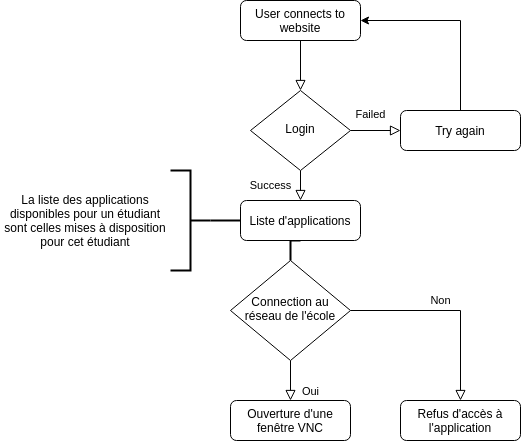
\includegraphics[scale=0.5]{images/VNC_use_case.png}
    \caption{Connexion au serveur}
    \label{fig:global_arch}
\end{figure}

\section{Plan du document}
Dans la suite de ce document, va être d'abord décrit les différentes recherches effectuées, les technologies appliquées et l'architecture de la distribution. 
Ensuite, nous allons aborder l'implémentation et les tests effectués sur la distribution.
La partie gestions de licences va être décrite avec les recherches et les décisions prises initialement.
Suite à une discussion avec un intervenant externe, il a été choisi qu'une direction autre que celle prise de base devra être suivie.
La phase de recherche et les décisions prises quant à cette direction sera explicitée.
Enfin, l'architecture, l'implémentation et les tests seront expliqués.
Finalement, une partie sera dédiée à l'analyse des résultats obtenus et une sur les travaux à réaliser et le futur de ce projet.




\chapter{Distribution}
\label{ch:distrib}


\section{Recherches}
Lors de cette partie du travail, une étude comparative a été effectuée pour essayer de trouver la base de distribution la plus adaptée aux besoins des utilisateurs de l'\textit{HEIG-VD}.
Tout d'abord, il a fallu évincer certaines distributions qui sont trop spécifiques, comme \textit{Kali Linux}, \textit{Parrot OS}.
En effet, certaines de ces distributions sont spécifiques au domaine de la sécurité et sont livrées avec beaucoup plus d'outils que nécessaire au bon fonctionnement d'un étudiant.
Il a alors été décidé de comparer les distributions principales :
\begin{itemize}
    \item Ubuntu
    \item Debian
    \item Manjaro
    \item Archlinux
\end{itemize}   
Le détail de cette comparaison se trouve ci-dessous :

\begin{figure}[H]
	\centering
	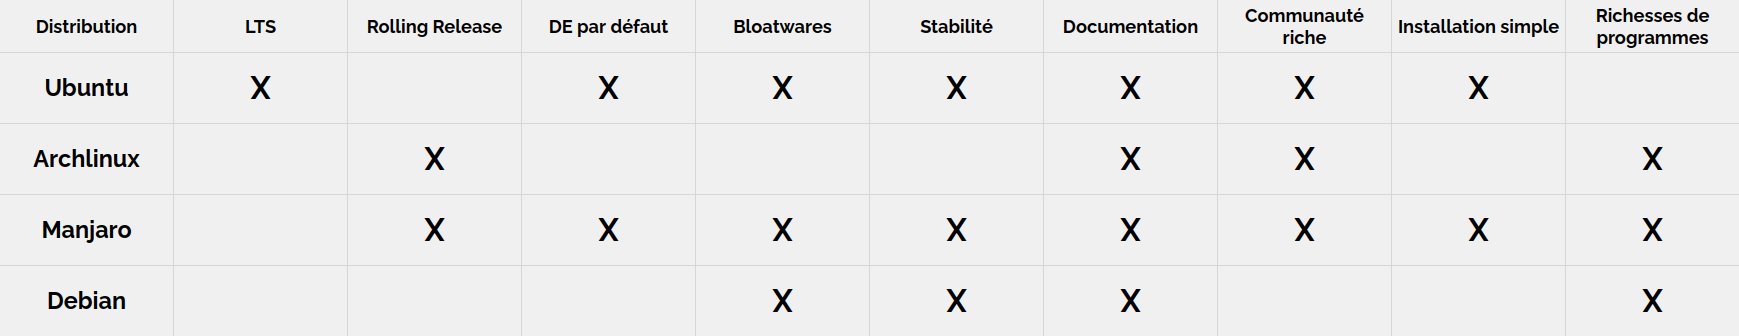
\includegraphics[scale=0.25]{images/distros_comp.png}
	\caption{Comparaisons des distributions}
	\label{fig:distros_comp}
\end{figure}


Le système de points est défini selon les critères suivants :
\begin{enumerate}
    \item Utilité
    \item Modularité
    \item Personnalisation
    \item Légèreté
\end{enumerate}

Finalement, Ubuntu est sorti comme choix de base de distribution. 
Le fait que cette distribution utilise un système de \acrfull{lts} permet de garantir une stabilité dans la compatibilité avec une multitude d'ordinateurs différents et ce de manière durable.
Les soucis principaux de cette distribution sont la surcouche \textit{\GLS{GNOME}} gérant le \acrfull{gui} et les logiciels installés de base.
Pour le dernier de ces problèmes, il a fallu trouver un moyen d'enlever un maximum de logiciels et librairies sans casser le système.
Au terme de certaines recherches, il a été déterminé que ces logiciels peuvent être ciblés et supprimés de manière aisée.
\newline
Concernant le soucis principal, l'utilisation de \GLS{GNOME}, il a fallu refaire une analyse comparative entre les \acrfull{de} principaux :
\begin{figure}[H]
	\centering
	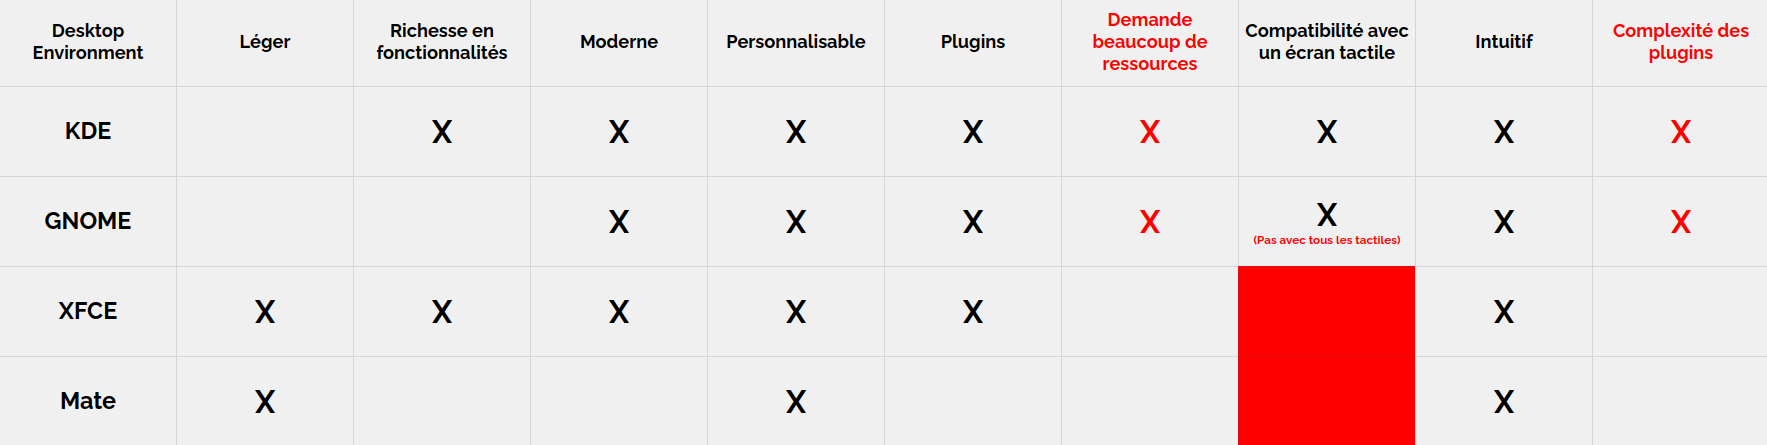
\includegraphics[scale=0.25]{images/DE_comp.png}
	\caption{Comparaisons des \acrfull{de}}
	\label{fig:de_comp}
\end{figure}
Il est possible de voir que seuls les principaux et les plus utilisés ont été mis en avant :	
\begin{itemize}
    \item KDE
    \item GNOME
    \item XFCE
    \item Mate
\end{itemize}
En effet, ces quatre \acrshort{de} font partie des plus utilisés et plus pratique pour un utilisateur lambda.
Il est en effet impératif de proposer une solution avec un \acrshort{gui} utilisable par n'importe quel utilisateur, c'est pourquoi des \acrshort{de} comme \textit{i3}, \textit{bspwm}, etc. ont été mis de côté.
Le système de points a été mis en place de manière à pouvoir classer de manière simple et efficace :
\begin{enumerate}
    \item Légèreté
    \item Efficacité
    \item Modularité
\end{enumerate}
Ces critères paraissent essentiels et peuvent englober plusieurs aspects différents, le tout permettant d'avoir un aperçu complet d'un \acrshort{de}.
Pour finir, il a été retenu que la surcouche \gls{GNOME} sera complètement supprimée de la base de distribution \textit{Ubuntu} et sera remplacée par \textit{XFCE}. 
\newline
Jusqu'à lors, il était relativement complexe de configurer les différents services de l'HEIG comme la connexion au réseau, le VPN, les imprimantes ou l'accès à \textit{eistore}.
L'idée serait de fournir une centralisation des identifiants HEIG afin de permettre la connexion aux services énoncés.
Grâce à une demande automatique du mot de passe lors du login, il sera alors possible de déverrouiller tous ces services et donc d'y accéder.
Un ajout potentiel pourrait être un script permettant de recevoir les notes présentes sur GAPS par message sur l'application Telegram.
Un aspect légal de cette proposition reste encore à voir.
L'API de Telegram permet de mettre en place un bot qui accepte les messages envoyés depuis un Terminal.
Sur ce bot, il est possible de récupérer certaines informations comme les notes d'une année en particulier, d'une matière en particulier ou même de mettre en place une tâche récurrente permettant d'avoir les différentiels à intervalle précis.


\section{Spécifications}

\subsection{Installateur}
Afin de pouvoir installer la distribution aux étudiants de l'HEIG-VD, un fichier \textit{.iso} sera fourni avec toutes les spécificités d'un installateur classique.
La distribution fournie sera configurée avec \textit{XFCE} et les logiciels superficiels seront désinstallés. 
\newline
Ensuite, afin de mettre le système courant sous forme ISO, \cite{ISO} il est possible de faire cela grâce à certaines commandes natives d'Ubuntu.

% TODO : Finir ça !!

\subsection{Scripts de centralisation}

Lors du premier démarrage après installation, un script Python fait une demande de saisie des identifiants AAI.
En effet, il est possible depuis Python de configurer des connexions aux réseaux grâce à \textit{nmcli}\cite{nmcli}.
Une connexion VPN peut être mise à disposition en utilisant l'écriture dans le fichier de configuration zsh, bash ou n'importe quel shell, créant ainsi un alias avec la bonne ligne de configuration.
L'utilisation de \textit{openconnect} comme VPN permet de simplifier l'accès au service.
La configuration de l'accès aux partages \textit{eistore} se fait de la même manière, un alias dans le fichier de configuration du shell.
Pour finir, les imprimantes peuvent être configurées grâce à l'outil \textit{lpadmin}. 
\newline
Le fait de faire une configuration comme cela permet d'éviter au maximum le stockage d'identifiants et de mots de passes.
Dans le cas des imprimantes et réseau sans fil, il n'y a pas d'autres alternatives que de configurer en dur dans le \gls{filesystem} la paire identifiants/mot de passe.
La localisation du stockage de ces derniers implique que seule une personne avec le mot de passe de la session et le mot de passe \textit{root} pourrait lire les informations.
Dans le cas des espaces \textit{eistore} et du VPN, le mot de passe sera demandé automatiquement lors de l'appel à ces alias et ne sera pas stocké sur l'ordinateur. 

\begin{figure}[H]
	\centering
	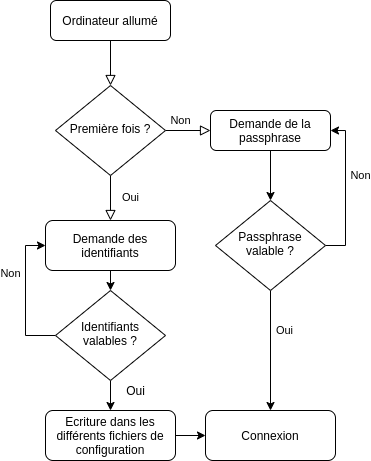
\includegraphics[scale=0.5]{images/centralisation.png}
	\caption{Demande des identifiants}
	\label{fig:central}
\end{figure}

\subsection{Notes et bot Telegram}
Pour cette partie, une configuration du bot existant \cite{bot} peut être configuré mais cela devra être fait manuellement.
Il est possible de fournir une automatisation du procédé de configuration mais elle ne parait pas optimisée ni sécurisée.
Pour se faire, il faut suivre la documentation fournie sur le dépôt mais qui va devoir être étoffée et complétée lors de ce travail.
Le bot est codé en Python et interagi avec Telegram grâce à l'API Telegram.
De plus, une discussion doit être engagée avec l'équipe s'occupant de Gaps, afin de pouvoir déterminer la légalité dans laquelle s'inscrit ledit script.

\section{Implémentation}

\subsection{Script de centralisation}
Ce script a pour but de configurer et faciliter l'accès aux différents services réseaux de l'HEIG-VD.
En effet, les imprimantes, les réseaux \textit{HEIG-VD} et \textit{eduroam}, le VPN et les dossiers partagés \textit{eistore}.
Le script complet se trouve en annexe et nous allons maintenant l'analyser.

\subsubsection{VPN}

\begin{listingsbox}{Python}{VPN}
file_path = expanduser("~/.zshrc")
file_object = open(file_path, 'a')
alias = "alias vpnHEIG=\"sudo openconnect --authgroup=All_Users --user=" +
username + " https://remote.heig-vd.ch\" \n"
file_object.write(alias)
\end{listingsbox}

Le script étant mis en place pour la distribution fournie lors de ce travail, il est assumé que l'utilisateur de ce script possède un terminal \textit{zsh}.
Cette partie du script écrit dans la configuration du terminal un alias qui permettra à l'utilisateur de lancer une connexion VPN vers le réseau de l'école.

\subsubsection{Réseaux}

Cette partie se décompose en deux fonctions :
\begin{itemize}
	\item la recherche de réseau
	\item la connexion au réseau
\end{itemize}

En effet, avant de pouvoir se connecter à un réseau, il faut vérifier qu'une connexion à ce réseau n'existe pas et si une interface réseau supportant le wifi soit disponible.

\begin{listingsbox}{Python}{Recherche de réseau}

\end{listingsbox}


\begin{listingsbox}{Python}{Connexion au réseau}
def connect(username, password, ext, network):
	command = "nmcli con edit id " + network
	method = "set ipv4.method auto"
	eap = "set 802-1x.eap peap"
	auth = "set 802-1x.phase2-auth mschapv2"
	mgmt = "set wifi-sec.key-mgmt wpa-eap"
	user = "set 802-1x.identity " + username + ext
	
	pwd = "set 802-1x.password " + password
	save = "save"
	acti = "activate"
	quit = "quit"
	
	child = pexpect.spawn(command)
	child.expect('nmcli>')
	child.sendline(method)
	
	child.expect('nmcli>')
	child.sendline(eap)
	
	child.expect('nmcli>')
	child.sendline(auth)
	
	child.expect('nmcli>')
	child.sendline(mgmt)
	
	child.expect('nmcli>')
	child.sendline(user)
	
	child.expect('nmcli>')
	child.sendline(pwd)
	
	child.expect('nmcli>')
	child.sendline(save)
	
	child.expect('nmcli>')
	child.sendline(acti)
	
	child.expect('Connection successfully activated')
	child.sendline()
	
	child.expect('nmcli>')
	child.sendline(save)
	
	child.expect('nmcli>')
	child.sendline(quit)
	
\end{listingsbox}

Cette fonction gère les interactions avec le client \textit{nmcli} de manière à pouvoir configurer la connexion correctement.
Il faut donc définir les protocoles à utiliser avec le \textit{peap}, la définition d'adresse ipv4 se fait automatiquement, et le fait de définir que la gestion de clés se fait via \textit{wpa-eap} permet de ne pas spécifier de certificats.
\newline
D'un point de vue de sécurité, il s'agit d'un non-sens que de fournir cette connexion car cela implique que les communications ne seront pas chiffrées.
Malheureusement, il s'agit ici de la politique de connexion de l'école.
En effet, pour les réseaux \textit{eduroam} et \textit{HEIG-VD}, l'école nous fournit une documentation qui nous spécifie de ne pas fournir de certificats.
Pour \textit{eduroam}, le site officiel nous fournit un script d'installation qui permet de retrouver un certificat.
Cette connexion sera donc configurée de manière sécurisée.

Suite à cela, les appels suivants sont faits afin d'établir les connexions :

\begin{listingsbox}{Python}{}
if checkNet("HEIG-VD"):
	connect(username, password, "@heig-vd.ch", "HEIG-VD")
else:
	print("no interface to work with")

if checkNet("eduroam"):
	connect(username, password, "@hes-so.ch", "eduroam)
else:
	print("no interface to work with")
\end{listingsbox}

\subsubsection{Imprimante}

\begin{listingsbox}{Python}{Imprimantes}
ppd_path = expanduser("~/driver/HEIG_Printer.ppd")
printer = "lpadmin -p FOLLOWME_PS -E -v smb://EINET/" + username + ":" +
 password + "@print.einet.ad.eivd.ch/FOLLOWME_PS -P " + 
 ppd_path + " -L \"HEIG-VD\" - o auth-info-required=negotiate"
process = subprocess.Popen(printer.split(), stdout=subprocess.PIPE)
\end{listingsbox}

Afin de configurer les imprimantes de manière supportée et homologuée par l'école, il faut passer par le client \textit{CUPS}.
Ce dernier permet une configuration via une ligne de commande : \com{lpadmin}.
Le soucis principal de cette manipulation réside dans le fait que la politique de l'école veut qu'un étudiant passe ses identifiants en clair et en dur dans l'URL de connexion.
Il n'existe aucun autre moyen de se connecter aux imprimantes, c'est pour cela que la configurations de ces dernières a été faite comme ceci.

\subsubsection{eistore}

\begin{listingsbox}{Python}{eistore}
create_eistore0 = "sudo mkdir /mnt/eistore0"
eistore0 = "sudo mount -v -t cifs -o domain=EINET,username=" + username + 
" //eistore0/softs /mnt/eistore0"
alias0 = "alias eistore0=\"" + eistore0 + "\"\n"
create_eistore1 = "sudo mkdir /mnt/eistore1"
eistore1 = "sudo mount -v -t cifs -o domain=EINET,username=" + username + 
" //eistore1/softs / mnt/eistore0"
alias1 = "alias eistore1=\"" + eistore1 + "\"\n"
	
file_object.write(alias0)
file_object.write(alias1)

file_object.close()
\end{listingsbox}

A l'instar du VPN, la commande pour avoir accès aux disques partagés se fait sur demande.
C'est pour cela que la configuration d'accès à \textit{eistore} est faite via un alias.
En effet, il est possible de monter un disque \textit{SAMBA} grâce à la commande \com{mount} de Linux.
Il suffit donc à l'utilisateur de rentrer son mot de passe lors de l'exécution de la commande en alias et il aura accès aux espaces partagés souhaités.


\subsection{Configuration de la distribution}
Lors de cette étape, il a fallu commencer par supprimer les \gls{bloatwares} présents sur Ubuntu, dont la liste exhaustive se trouve en annexe de ce document.
Suite à cela, il a fallu enlever le \acrfull{de} \Gls{GNOME} afin de le remplacer par \textit{XFCE}.
L'installation de certains outils permettant d'exécuter le script de centralisation était aussi nécessaire.
Ensuite, la compression en \textit{.ISO} se fait via le \gls{filesystem} \textit{squashFS} et la conversion vers un installeur avec l'outil : \textit{Linux Live Kit}.

% TODO : Compléter avec la suite de la distro !!

\section{Tests}



\chapter{Gestion de licences}
\label{ch:softs}


\section{Recherches initiales}
Lors de cette première partie de recherches, il a fallu réfléchir au problème des différentes étapes de l'ouverture et d'utilisation d'une application.
En effet, il a fallu découper les étapes à sécuriser et c'est pour cela que les recherches effectuées se sont axées autour de l'ouverture de l'application et des interactions de cette dernière avec le \gls{filesystem} de l'application.

\subsection{Ouverture d'une application}
Lors de l'analyse faite lors de cette première partie, il a fallu définir un use-case satisfaisant pour le comportement à adopter lors de l'ouverture d'une application.
En effet, il devait être déterminer quelle technologie sera utilisée pour containeriser une application.
La discussion s'axait autour de la virtualisation et l'émulation, deux procédés de simulation distincts.
Afin de bien définir chacun des termes, il est impératif de faire un détour pour ne pas se méprendre sur les termes employés : 

\begin{itemize}
	\item Simulation : "Représentation fictive de la réalité. Il s'agit d'imiter [et modéliser] une situation"\cite{sev}.
	\item Emulation : "Procédé permettant de reproduire à l'identique le comportement d’un logiciel et son architecture matérielle." \cite{sev} Il est donc possible de simuler une architecture différente de celle installée sur la machine.
	\item Virtualisation : Procédé de virtualisation utilisant les ressources physiques de l'ordinateur. Il n'est donc pas possible de simuler une architecture différentes de celle présente sur la machine.
\end{itemize}
 
Au terme de ces recherches, il a été possible d'établir une liste de points positifs et négatifs pour chacune de ces technologies.

Concernant l'émulation :
\begin{itemize}
	\item Avantages :
	\begin{itemize}
		\item Une machine entière peut être construite depuis un logiciel
		\item Les composantes hardware peuvent être construites de manière logiciel
		\item Possibilité d'émuler des architectures vétustes (PowerPC par exemple)
	\end{itemize}
	\item Inconvénients :
	\begin{itemize}
		\item Gourmand en ressources
		\item Exécution de code étranger au niveau du kernel et CPU en le convertissant en ASM
	\end{itemize}
\end{itemize}
Concernant la virtualisation :
\begin{itemize}
	\item Avantages :
	\begin{itemize}
		\item Meilleures performances car moins de compilation
		\item La virtualisation se fait directement sur le hardware natif
	\end{itemize}
	\item Inconvénients :
	\begin{itemize}
		\item Limitations au niveau du hardware car il est impossible de virtualiser une architecture qui n'est pas présente
	\end{itemize}
\end{itemize}
\cite{evs}
\cite{evs2}
\newline

% TODO : Faire des schémas pour l'émulation et virtualisation

Au fur et à mesure de l'avancement du travail, la virtualisation est ressortie comme le choix définitif de technologies de simulation.
Cela est dû au fait qu'il s'agit d'une technologie plus optimisée au niveau des ressources utilisées.
En effet, il faut impérativement que l'utilisation de ces applications soit la plus optimisée et fluide possible, et ce malgré la surcouche utilisée.
\newline
Suite à cela, il a fallu choisir une technologie, utilisant la virtualisation, permettant d'afficher l'interface graphique d'une application.
Quatres technologies sont ressorties, QEMU, Docker, Kubernetes et snap.
Docker permet de créer un environnement Linux complet, permettant donc d'installer et de gérer un \gls{filesystem} à part.
De plus, Docker permet de construire une image qui sera ensuite reproductible, ce qui permet d'avoir plusieurs instances de la même image en même temps.
Ce comportement est très avantageux dans la construction de notre architecture.
\newline
QEMU permet d'avoir des performances optimisées sur des petits systèmes ou de tailles moyennes.
Tous les aspects de la virtualisation sont optimisés. 
Cependant, au niveau de l'installation et la prise en main, cet outil est beaucoup plus complexe que les autres outils.
Le maintien d'un tel outil peut s'avérer plus complexe que certains autres outils. 
\newline
Kubernetes se veut être le nouveau Docker car les deux technologies utilise la containerisation afin de gérer une application.
Kubernetes permet d'abstraire certaines parties du procédé de containerisation, ce qui rend son utilisation plus légère.
Le soucis est que de par son abstraction, sa gestion avec le \gls{filesystem} peut être moins facile et malléable qu'avec Docker
Les deux technologies peuvent être utilisées ensemble sans soucis.
En effet, les outils peuvent être complémentaires et la combinaison des deux est très performante.
\newline
Snap permet de containeriser des application à travers un packet manager mais n'offre pas de \gls{filesystem} et ne permet pas de personnaliser le container à notre volonté.
De plus, selon beaucoup d'experts, snap ne doit en aucun cas être utilisé sur des systèmes comme Archlinux car il installe beaucoup de composantes inutiles.
Dans l'idée que le projet doit être portable, il faut qu'un utilisateur utilisant n'importe quel \gls{Operating System} puisse lancer une application containerisé.
\newline
Finalement, l'outil Docker a été choisi car c'est celui qui offre les performances les plus complètes et qui a un support et une communauté les plus fournis.
De plus, de part la maîtrise plus prononcée de Docker et sa maniabilité, il est apparu évident de choisir cet outil.
Docker permet d'avoir un \gls{filesystem} externe à celui natif et d'interagir avec ce dernier.


\subsection{Interactions avec le filesystem}

Après analyse des différents scénarios, il est apparu qu'il fallait aussi gérer les interactions avec le \gls{filesystem} entre le container et le natif.
L'idée recherchée était de mettre en place un système permettant d'écrire sur le système natif seulement si le fichier modifié est authentifié comme travail de l'école.
Dans ce but, il est nécessaire de créer un système de signatures de fichiers qui émet un signal au \gls{filesystem} que le container peut écrire.
Cela implique que les professeurs devront mettre en place un système de distribution de fichiers qui seront authentifiés au préalable.
L'idée serait de mettre en place une autorité de vérification qui peut signer les fichiers envoyés sur le serveur.
Avec ce système, le container Docker ne pourrait écrire sur le \gls{filesystem} natif si et seulement si la signature est valable.
Si la signature est valable, un signal sera envoyé au Docker et lui permettra d'écrire de manière persistante les données de l'utilisateur.
Pour ce faire, il est possible d'implémenter un script Python qui gère l'envoi et la réception des signaux système et qui communique avec le \gls{filesystem} du container Docker.
\newline
Lors d'un point de situation hebdomadaire, M. Kapfer a mis en avant des soucis de sécurité avec l'approche prise jusqu'à maintenant.
En effet, l'utilisation de Python dans la gestion des interactions avec le \gls{filesystem} peut poser des problèmes de modifications du script.
En effet, Python n'étant pas un langage compilé, il est possible de retrouver le code source du script et donc de le modifier.
De plus, il évoque la complexité de créer une autorité de signatures et le problème de vérification du fichier signé.
\newline
Une solution aurait été de mettre les scripts d'installation dans un dossier appartenant à un utilisateur système, dont personne n'a le mot de passe, et qui n'a aucun droit sur le système à part l'exécution de ces scripts.
Cela aurait complexifié les interactions au niveau du \gls{filesystem} et du container Docker.
De plus, aucune solution n'a permis de simplifier la création de l'autorité de certification.
\newline
Une autre solution, suggérée par M. Kapfer, serait d'utiliser une infrastructure client-serveur qui communique à travers une technologie \acrshort{vnc}.
Le serveur aurait une partie disque propre à chaque étudiant ou professeur.
Les applications ne seraient pas installées sur l'ordinateur de l'étudiant mais sur le serveur et accessible via un client Web.
\newline
Au terme de plusieurs discussions et réflexions, il apparaît clairement que cette dernière approche est celle à choisir.
Le système de lancement d'application resterait le même, mais serait déporté sur un serveur distant.
\newline
Avec l'adoption de cette approche, il est impératif de savoir si l'utilisation de la technologie \acrshort{vnc} sur un client Web.
En regardant sur différents types d'articles, il est ressorti qu'il était possible de faire une telle action en utilisant un serveur CentOs.\cite{vnc}
L'utilisation d'une telle distribution Linux permet de pouvoir gérer plus facilement certains aspects de droits utilisateurs sur un fichier.
En effet, la configuration des \acrfull{acl} et des permissions classiques permet de pouvoir gérer les droits de modification, de lecture. d'ajout, de suppression et bien d'autres sur un fichier ou un dossier.
De ce fait, il est possible d'envisager que sur le serveur, un utilisateur puisse effectuer une action et un autre ne le puisse pas.
Cela permettra de mettre en place des rôles distincts pour les professeurs et pour les étudiants.
\newline
Il est possible de rajouter une couche de sécurité pour gérer les aspects de containerisation du tunnel \acrshort{vnc}.
Un servlet du nom de \textit{Guacamole} permet de diffuser une fenêtre \acrshort{vnc} pour un utilisateur donné avec une paire "username:password".

\section{Spécifications}

\subsection{Configuration du serveur}
Lors de la configuration du serveur, il faut installer une version de CentOs 7.
Une autre version ne permet pas l'installation "simple" de certaines composantes essentielles telle que \textit{php5.5}, \textit{guacamole} pour ne citer qu'elles.
Il est nécessaire d'avoir une interface graphique pour faire marcher le \acrshort{vnc} de manière correcte.
Une fois le serveur installé, il faut configurer les différents composantes permettant de mettre en place le \acrshort{vnc}.
Il faut donc installer le \acrshort{vnc} Server \cite{vncs} permettant d'indiquer au client qu'il faut regarder à un endroit donné du \gls{filesystem}.
Sur ce serveur, il faut distinguer trois rôles distincts :
\begin{itemize}
	\item Admin
	\item Teacher
	\item Student
\end{itemize}
En effet, chaque rôle pourra faire des actions différentes.

\begin{figure}[H]
	\centering
	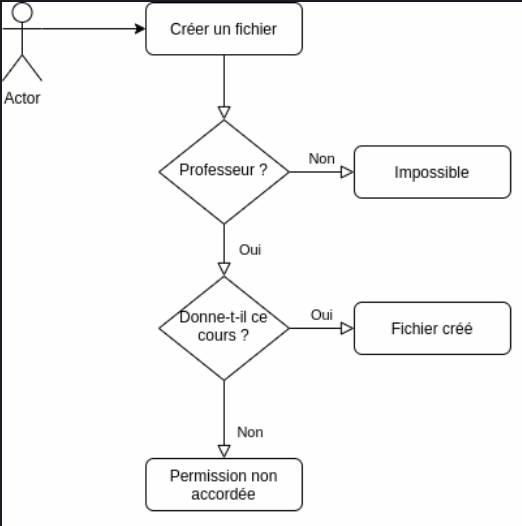
\includegraphics[scale=0.45]{images/create.png}
	\caption{Création de fichiers}
	\label{fig:create}
\end{figure}


\begin{figure}[H]
	\centering
	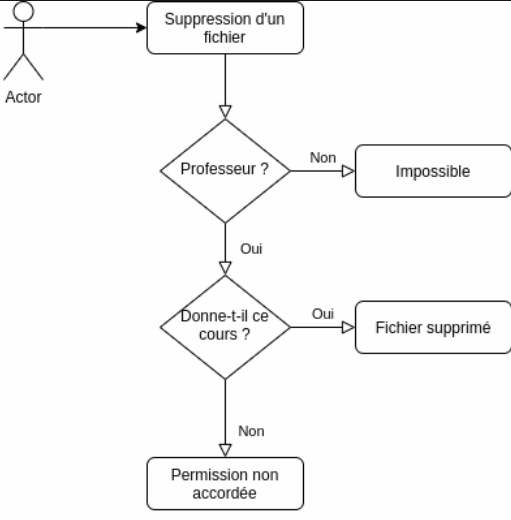
\includegraphics[scale=0.45]{images/delete.png}
	\caption{Suppression de fichiers}
	\label{fig:delete}
\end{figure}


\begin{figure}[H]
	\centering
	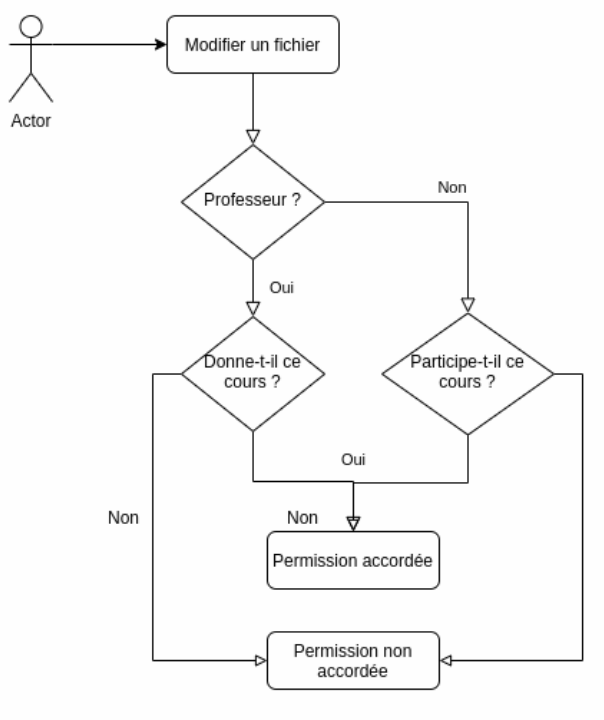
\includegraphics[scale=0.45]{images/edit.png}
	\caption{Modification de fichiers}
	\label{fig:edit}
\end{figure}


\begin{figure}[H]
	\centering
	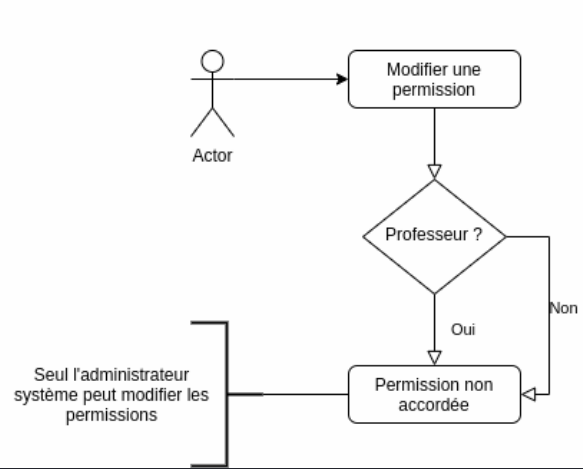
\includegraphics[scale=0.45]{images/perms.png}
	\caption{Modification des permissions}
	\label{fig:perms}
\end{figure}

L'administrateur peut évidemment modifier, rajouter et supprimer des fichiers.
\newline
Toute ces cas peuvent s'appliquer grâce à l'utilisation d'une base de données, en \textit{PostgresQL} par exemple.
% TODO : Vérifie le graph SQL pour ne rien oublier !
La base de données est très simple et comprend quatre tables comme présenté ci-dessous :
\begin{figure}[H]
	\centering
	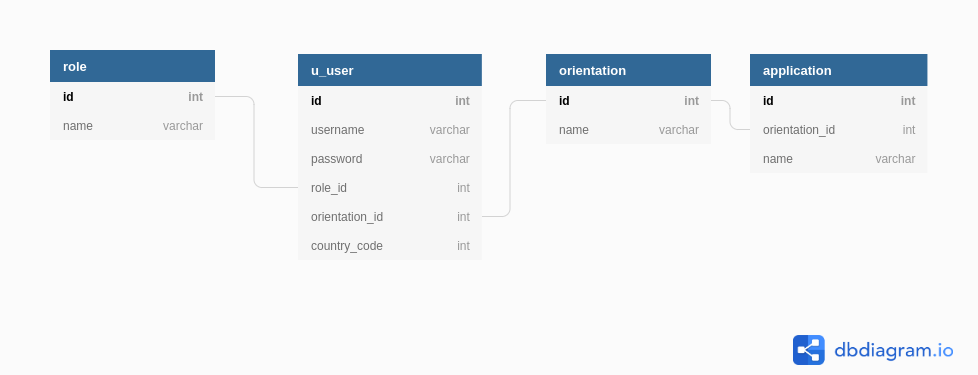
\includegraphics[scale=0.45]{images/DB.png}
	\caption{Base de données}
	\label{fig:db}
\end{figure}
L'utilisation de cette base de données permet de créer un espace utilisateur pour chacun des étudiants ou professeurs présents dans la table \textit{u\_user}.
En fonction de l'orientation d'un utilisateur, une liste d'applications lui est attribuée.
Un dossier est créé pour chaque application avec un script bash de lancement à l'intérieur.
Lors de la création d'une connexion sur le client Web, ce dernier appellera le script correspondant à l'application souhaitée.


\subsection{Client Web}
Le client Web a pour but de donner une fenêtre de lecture aux étudiants, leur permettant de choisir les applications à lancer depuis leur navigateur.
L'accès à ce site sera protégée et accessible avec les identifiants AAI. 
De ce fait, il est possible d'utiliser la technologie php pour aller faire les vérifications sur la base de données créée au préalable.
Ensuite, une liste d'applications, propre à chaque étudiant, sera dressée et avec une simple sélection de l'application.
Une interface utilisateur permet de voir le nombre d'applications disponibles pour chaque étudiant, de voir l'espace disque disponible sur le serveur et une liste de devoirs mise à disposition par les professeurs.
Tout le code mis en place dans cette partie sera fait en \textit{HTML5}, \textit{CSS3}, \textit{PHP} et \textit{Javascript}.
Le flot général sur le site est le suivant :
\begin{figure}[H]
	\centering
	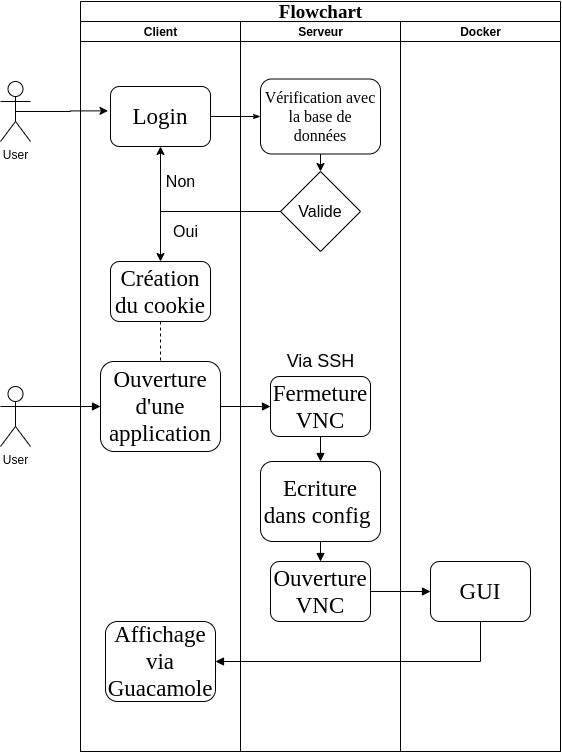
\includegraphics[scale=0.35]{images/client_flow.png}
	\caption{Flot des actions sur le site lors de l'ouverture d'une session et d'une application}
	\label{fig:client_flow}
\end{figure}

\subsection{Ouverture de l'application}
Lors de la phase d'ouverture, après la sélection de l'utilisateur dans son navigateur, tout se passe du côté du serveur.
La sélection utilisateur permet de déclencher un appel à un script bash qui lancera l'application containerisée avec Docker.
L'image du container sera construite au préalable mais le script vérifiera quand même si tel est bien le cas.
Ensuite, il faut configurer le \acrshort{vnc} pour qu'il ne diffuse que la fenêtre entrain de se lancer et pas de fenêtres de Terminal ou de gestionnaire de fichiers.
Lors de l'appel par le client Web, le serveur \acrshort{vnc} exécuté sur le serveur pour un étudiant est arrêté, le fichier de configuration modifié de sorte à lancer la bonne application et relancé pour enfin diffuser l'application sur le client.

\begin{figure}[H]
	\centering
	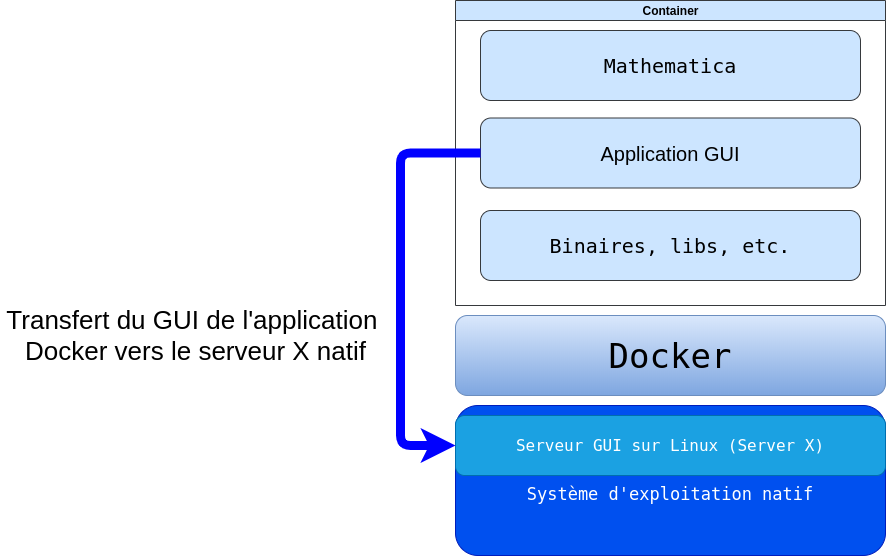
\includegraphics[scale=0.35]{images/container.png}
	\caption{Container Docker avec application GUI}
	\label{fig:cont}
\end{figure}


%TODO : Faire un schéma du script !
\subsection{Containerisation des application}
Afin de containeriser une application, il est nécessaire de créer un Dockerfile définissant les règles de construction de cette dernière.
Il est, à priori, impossible d'automatiser ce processus car chaque application demande des pré-requis spécifiques.
En revanche, une base commune permet de comprendre et de rendre l'écriture de ces fichiers de configurations et de rendre le lancement plus simple.
En effet, les applications arrivent à se lancer en mode GUI grâce à un partage de ressources avec l'aide d'un volume.
Il faut mettre en commun la ressource graphique de la machine hôte et passer en variable d'environnement le numéro de "display", par défaut \textit{:0}.
De ce fait, il est possible d'établir un \textit{template} avec les lignes directrices du Dockerfile mais pas de généraliser sa construction.
De par la configuration du serveur, il est impossible pour le Docker de traverser les dossiers, ce qui rend l'écriture dans une autre partie impossible.
De plus, Docker ne peut pas créer ou supprimer des fichiers, seulement modifier un fichier existant, grâce à la configuration du serveur.
Chaque application aura un container séparé, ce qui limite les risques d'intrusion et d'interactions non-contrôlées.
Les containers ne seront pas atteignables depuis l'extérieur du réseau du serveur.
Cela permettra de limiter encore une fois la surface d'attaque depuis l'extérieure.

\subsection{Interactions avec le filesystem}
Les interactions entre le \gls{filesystem} du container et le \gls{filesystem} natif doivent être régulées selon les figures \ref{fig:create} \ref{fig:delete} \ref{fig:edit} \ref{fig:perms}.
Cela peut être grâce aux configurations des ACLs sur le serveur.
Ce procédé suffirait à garantir qu'aucun étudiant ne pourrait utiliser les logiciels fournis par l'école de manière illicite.
Les professeurs fournissent le fichier sur l'espace personnel des étudiants et les étudiants ne peuvent que modifier le fichier en question.
Il n'est alors plus nécessaire d'avoir une gestion des actions à l'intérieur même du container Docker.
De même façon qu'un utilisateur ne pourra pas rajouter de fichiers sur son \gls{filesystem}, Docker ne pourra pas le faire non plus.
Docker doit pouvoir prendre les fichiers présents dans le dossier et doit pouvoir écrire seulement si le fichier existe au préalable.
Cela est réalisable lors du \textit{run} du container Docker. 
Le fait de partager un volume entre le \gls{filesystem} natif et celui du Docker permet de garantir qu'il n'y aie pas de modifications à un autre endroit que sur le dossier partagé.

\section{Architecture}
\begin{landscape}
	\begin{figure}[H]
		\centering
		\includegraphics[scale=0.55]{images/VNC&server_1.png}
		\caption{Architecture et comportement}
		\label{fig:arch1}
	\end{figure}
	\begin{figure}[H]
		\centering
		\includegraphics[scale=0.55]{images/VNC&server_2.png}
		\caption{Architecture et comportement}
		\label{fig:arch2}
	\end{figure}
	\begin{figure}[H]
		\centering
		\includegraphics[scale=0.55]{images/VNC&server_3.png}
		\caption{Architecture et comportement}
		\label{fig:arch3}
	\end{figure}
		
\end{landscape}

\section{Implémentation}

\subsection{Docker}

Afin de créer un container avec GUI, il est nécessaire de transférer l'environnement graphique du container vers celui de l'ordinateur hôte. 
Cela consiste à signaler au Docker qu'il doit utiliser une ressource partagée via le Dockerfile. 
Dans le Dockerfile ci-dessous, il est possible de voir qu'une variable d'environnement \com{ENV DISPLAY :0} est passée au container.
Cette variable permet de signaler le composant graphique à utiliser par le container.
\newline
Ensuite, il faut savoir quelles sont les dépendances du programme à installer et donc les passer en commande de construction du container.
Afin de minimiser la taille de l'image, il faut concaténer autant que possible les commandes ensemble. 
En reprenant le Dockerfile ci-dessous, il est possible de dégager certaines parties essentielles du fichier.
\newline
La première ligne sert à définir la version d'Ubuntu à utiliser.
Dans le cas actuel, il est recommandé d'utiliser Ubuntu 18.04.
Ensuite, il est nécessaire de copier tous les fichiers d'installation vers le container.
Il est possible de les placer dans un dossier arbitraire, mais recommandé de les mettre dans \com{/data}.
\newline
Les commandes des lignes 7 et 8 servent à définir la zone géographique du container.
Cette étape n'est pas nécessaire dans la majorité des cas mais dans le cas de Mathematica, il est obligatoire de le faire.
Ensuite, il est obligatoire d'installer les mises à jour et la commande  \com{sudo}.
Efin, il est recommandé de créer un utilisateur lambda, \textit{user} dans le cas actuel, afin de ne pas donner tous les droits à l'utilisateur final.
Après avoir créé cet utilisateur, il faut finalement installer toutes les dépendances de l'application. 
C'est à cause de cette partie qu'il est impossible de rendre la création des Dockerfile générique.

\inputsourcecode{bash}{"source_code/Dockerfile"}{Dockerfile}

Une fois le Dockerfile écrit, il est possible de lancer un script permettant de lancer le container.
Ce script permet de regarder dans le \gls{filesystem} natif si l'image a déjà été construite.
Si l'image est déjà construite, le script ne fait qu'appeler \com{docker run}.
Dans le cas où l'image n'est pas construite, il est impossible de construire l'image depuis un espace étudiant.
Seuls les professeurs ou les administrateurs pourront avoir accès au Dockerfile.

\inputsourcecode{bash}{"source_code/launch.sh"}{launch.sh}

L'appel à \com{docker images -q john:doe} permet de savoir si l'image existe ou non.
\begin{listingsbox}{console}{Docker images}
user@user:~$ docker images -q fsmdbfsdnfdssdhfsd:asashdalk
user@user:~$
\end{listingsbox}
La sortie de l'appel à cette fonction sera vide si l'image n'existe pas.
\newline
Si l'image existe, l'identifiant sera en sortie :


\begin{listingsbox}{console}{Docker images}
user@user:~$ docker images -q test:latest
7d7d5f60428a
user@user:~$
\end{listingsbox}

Lors de l'appel à \com{docker run}, il faut préciser où se trouve l'instance de Server X sur l'ordinateur hôte et de créer un volume partagé entre le container et l'hôte.
\newline
Les exemples utilisés pour ce travail sont Mathematica, comme montré ci-dessus, et Logisim qui se trouvera en annexe.
La raison pour laquelle il a été choisi de prendre ces logiciels comme exemple est que l'un est un logiciel demandant beaucoup de ressources matérielles pour certains calculs et l'autre est utilisé de manière concrète lors de certains cours donnés par le \textit{REDS}.


\subsection{Configuration du serveur}

Afin de configurer le serveur, le service informatique de l'école avait été contacté. 
Il aurait été souhaitable d'avoir une machine virtuelle sur les serveurs de développement de l'école afin de pouvoir travailler en conditions de production.
Malheureusement, la configuration graphique du serveur n'a pas pu être possible et malgré la communication avec le responsable, une solution n'a pas pu être trouvée.
\newline
De ce fait, afin de simuler au plus proche possible le serveur, tout le travail a été fait sur machine virtuelle.
Après l'installation de CentOs 7, il a fallu créer une base de données en PostgresQL.
A l'aide de la requête ci-dessous, il est possible de récupérer les informations suivantes : 
\begin{itemize}
	\item Username
	\item Password
	\item Rôle
	\item Applications
	\item id
\end{itemize}

\begin{listingsbox}{SQL}{Requête}
SELECT u.username, u.password, r.role_name, 
array_to_string(array_agg(a.name), ',') AS Applications, u.user_id 
FROM u_user u INNER JOIN role r ON u.role_id = r.role_id 
INNER JOIN orientation o ON u.orientation_id = o.orientation_id 
INNER JOIN application a ON a.orientation_id = o.orientation_id 
GROUP BY u.user_id, u.username, u.password, r.role_name;
\end{listingsbox}

La spécificité de cette requête est cette partie : \com{array\_to\_string(array\_agg(a.name), ',')}. 
La première partie crée un tableau depuis la valeur des noms d'applications qui sont en commun avec la cause \textit{GROUP BY} de la fin de requête.
Une fois ce tableau créé, il est transformé en chaîne de caractères pour qu'il soit lisible dans les scripts suivants : 

\inputsourcecode{bash}{"source_code/.env"}{.env}
\inputsourcecode{bash}{"source_code/update_csv"}{update\_csv}
Les options utilisées pour appeler la base de données et l'exporter en \textit{.csv} sont les suivantes : 
\begin{itemize}
	\item \com{-t} : Supprime les noms de colonnes
	\item \com{-A} : Supprime l'alignement
	\item \com{-h} : Le nom de l'hôte de la base de données
	\item \com{-p} : Numéro de port
	\item \com{-d} : Nom de la base de données
	\item \com{-U} : Nom d'utilisateur de la base de données
	\item \com{-c} : Commande à exécuter
\end{itemize}

Avec le script situé dans le même dossier, \com{create\_user}, il est possible de lire le \textit{.csv} créé et d'ajouter un nouvel utilisateur si le fichier a été modifié.

\inputsourcecode{bash}{"source_code/create_user"}{create\_user}

Les deux scripts sont appelé dans le script \com{main} qui doit être appelé avec un utilisateur avec les droits \com{sudo}.
Une façon d'enlever les demandes de mots de passe et d'ajout de la commande \com{sudo} est d'ajouter l'exécution de la commande \com{main} dans les \textit{sudoers} et d'ajouter un alias pour enlever le \com{sudo}.

\inputsourcecode{bash}{"source_code/main"}{main}

\begin{listingsbox}{bash}{sudoers \& alias}
# Dans les sudoers
jeremy ALL=(root) NOPASSWD: /home/jeremy/docker/main
# Dans la configuration du terminal (bash, zsh, etc.)
alias main='sudo /home/jeremy/docker/main'
\end{listingsbox}
Bien évidemment, il faudra remplacer le chemin d'accès au script avec le bon chemin.


\subsection{Configuration de guacamole}

Afin de configurer le servlet Guacamole, il a fallu suivre le tutoriel de Deviant Engineer \cite{guac}.
Après la configuration initiale, il a fallu créer un alias et ajouter \com{guacd} aux sudoers car il était impossible de lancer le servlet sans cette manipulation.
\begin{listingsbox}{bash}{sudoers \& alias}
# Dans les sudoers
jeremy ALL=(root) NOPASSWD: /usr/local/sbin/guacd -f
# Dans la configuration du terminal (bash, zsh, etc.)
alias guacd='sudo /usr/local/sbin/guacd -f &'
\end{listingsbox}
Une fois le daemon lancé, il a fallu configurer le serveur \acrshort{vnc}.
Pour ce faire, il est nécessaire d'installer \textit{Tiger VNC}.
Sur CentOs, il a suffi de suivre le tutoriel proposé par Pradeep Kumar \cite{vnc_conf}.
Ensuite, comme montré dans le scripte "\textit{create\_user} ci-dessus, il est obligatoire de configurer correctement les fichiers d'utilisateurs de guacamole, situé dans \com{/etc/guacamole/user-mapping.xml}.
\begin{listingsbox}{xml}{Exemple d'utilisateur dans user-mapping.xml}
<authorize username="jeremy" password="pass">
	<protocol>vnc</protocol>
	<param name="hostname">localhost</param>
	<param name="port">5901</param>
	<param name="password">polopolo</param>
</authorize>
\end{listingsbox}
Le nom d'utilisateur et le mot de passe sont donnés de manière arbitraire et permettent d'identifier un utilisateur sur le client.
Le protocole doit être spécifié car il est possible de faire du \textit{RDP}, du \textit{SSH}, \textit{VNC} ou du \textit{Telnet}.
Le nom de l'hôte correspond à l'adresse sur laquelle le serveur \acrshort{vnc} a été configuré.
Le numéro de port doit être le même que celui ouvert par le serveur \acrshort{vnc}.
Enfin, le mot de passe est celui défini lors de la configuration du serveur \acrshort{vnc}.
\newline
De manière à rendre le serveur Guacamole opérationnel, il est nécessaire de faire un appel à l'alias créé au préalable.
\begin{figure}[H]
	\centering
	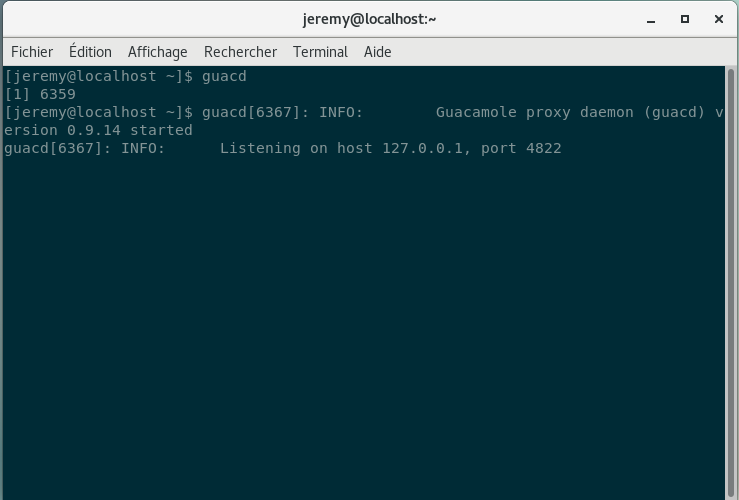
\includegraphics[scale=0.55]{images/guacd.png}
	\caption{Appel à \com{guacd}}
	\label{fig:guacd}
\end{figure}

Le client est accessible à l'adresse suivante : \com{localhost:8080/guacamole}.
\begin{figure}[H]
	\centering
	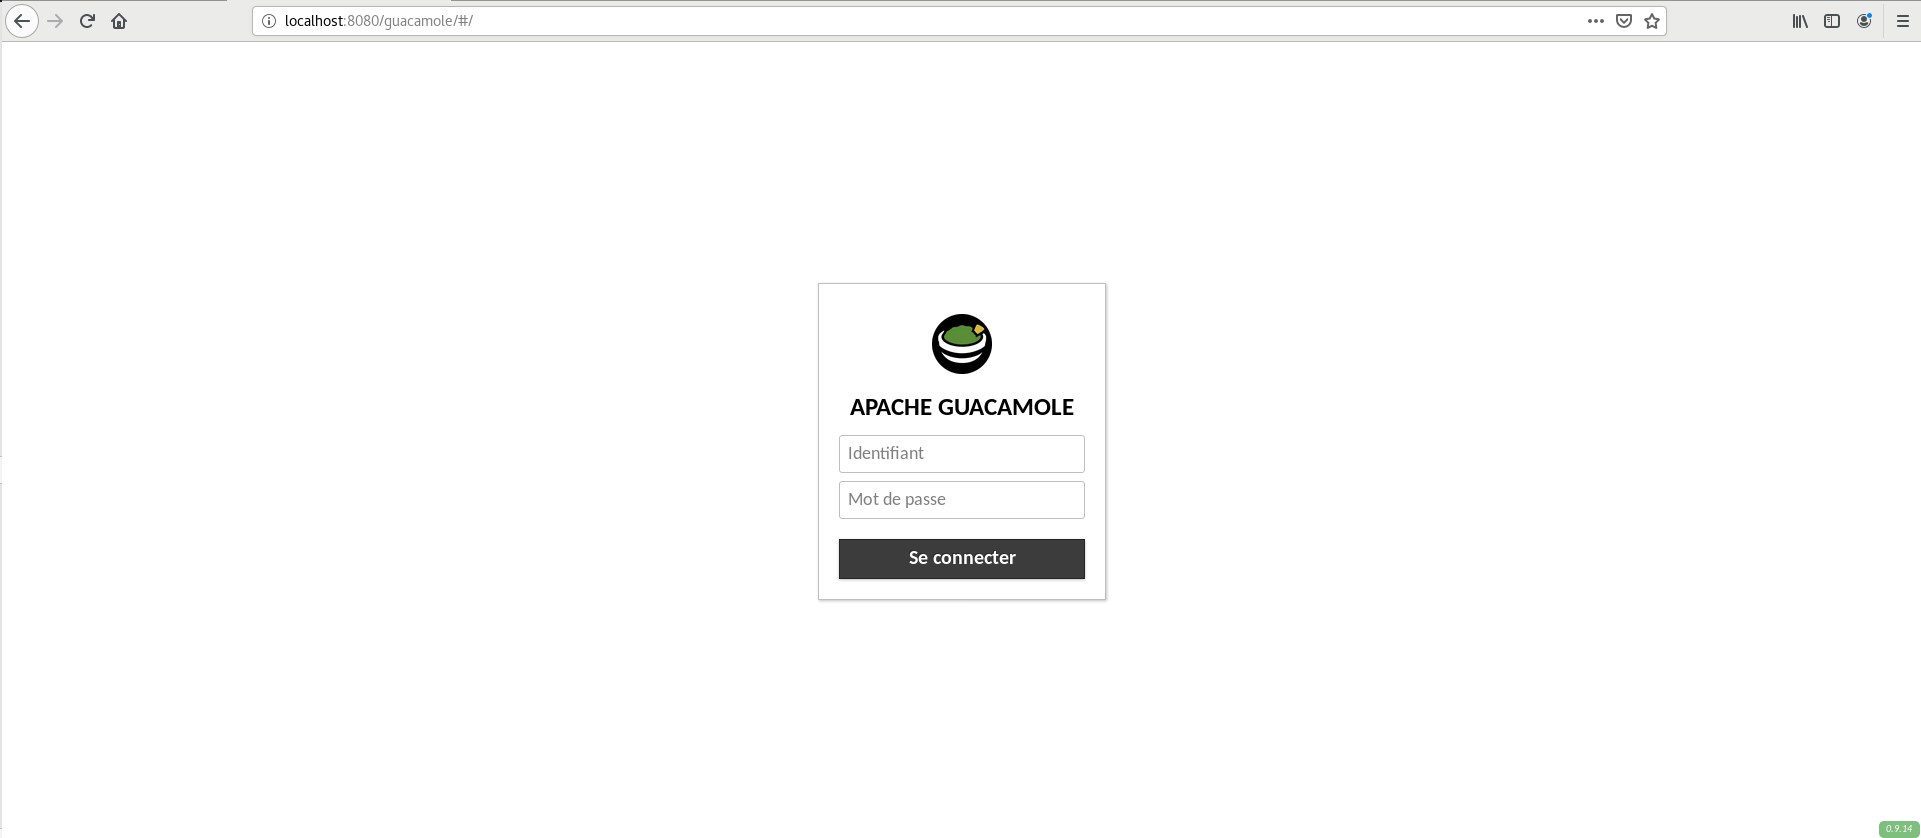
\includegraphics[scale=0.2]{images/guacd_client.png}
	\caption{Page d'accueil de Guacamole}
	\label{fig:guacd_client}
\end{figure}

\subsection{Site internet}
Pour commencer le développement du site, un template libre de droit a été trouvé sur le site de Creative Tim \cite{creatim}.
Une fois le site copié, il était possible de personnaliser l'interface utilisateur au bon vouloir du projet.
Il a fallu rajouter un accès à la base données et pour ce faire, la base de données créée lors de la configuration du serveur a été réutilisée.
\newline
En utilisant la technologie \textit{php-pqsql}, il est possible de faire des requêtes sur une base de données en Postgres avec l'aide de PHP.
Par exemple, pour établir une connexion, il suffit de faire : 
\inputsourcecode{bash}{"source_code/conn_db.php"}{Connexion à la base de données via PHP}
\begin{figure}[H]
	\centering
	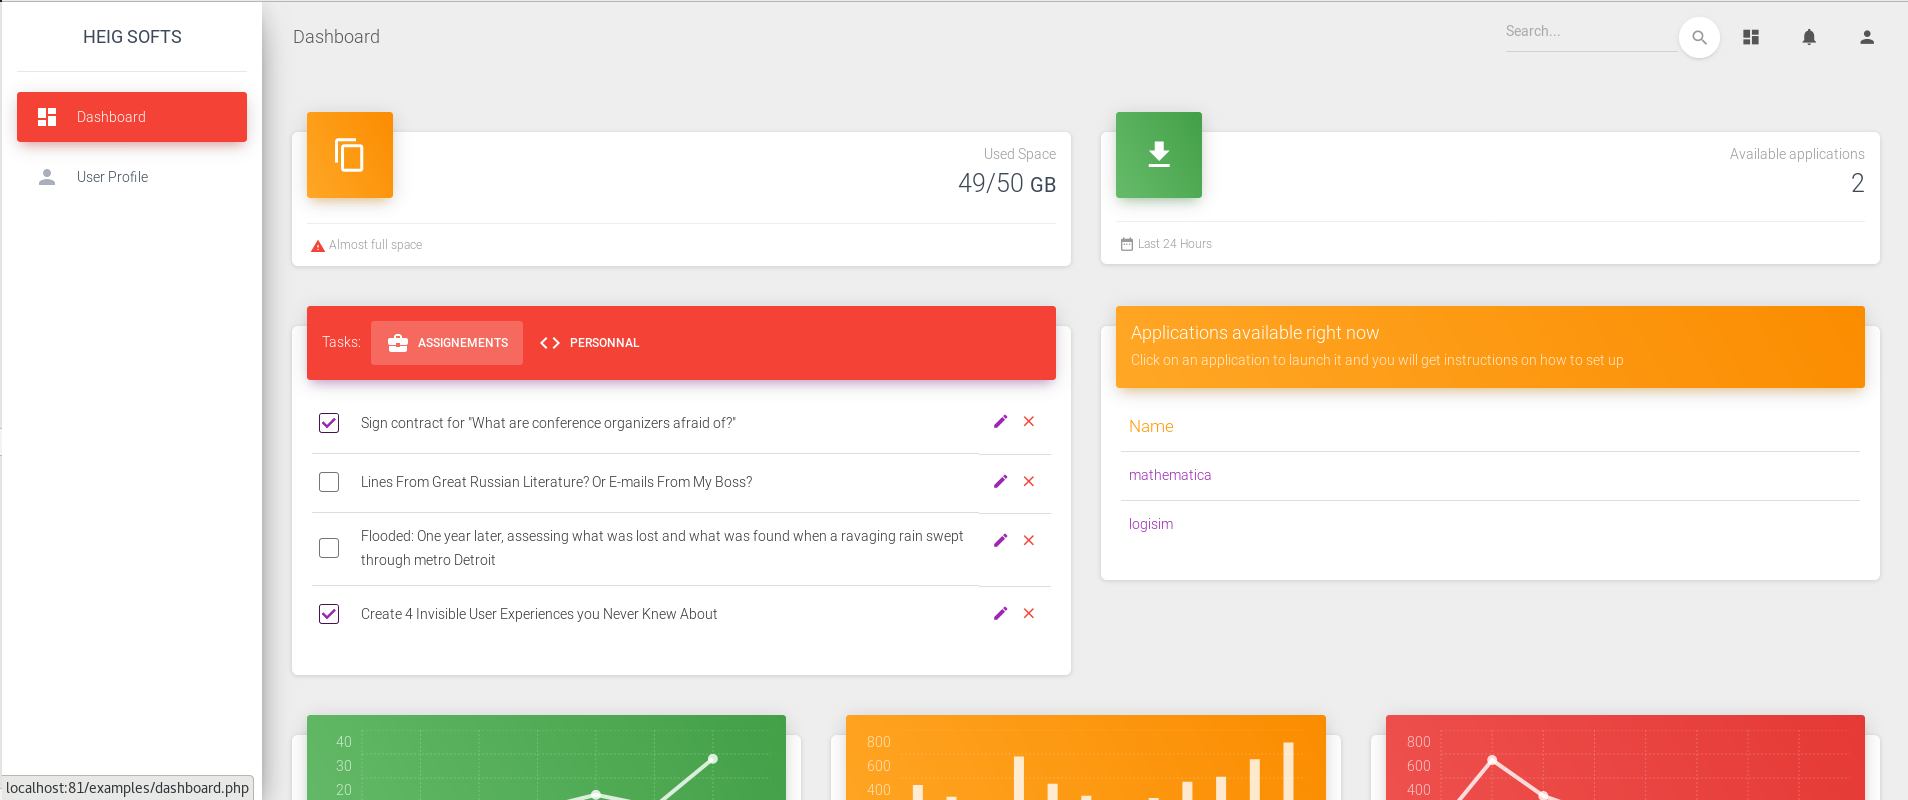
\includegraphics[scale=0.2]{images/website.png}
	\caption{Page d'accueil du site}
	\label{fig:website}
\end{figure}
Le site prend l'aspect d'un tableau de bord. 
Sur la droite apparaissent les applications disponibles. 
En cliquant sur l'une d'elles, il est possible d'accéder à la page d'affichage de l'application.
Sur la gauche se trouve une liste de devoirs mis à disposition par le professeur.
Pour le moment, cette fonctionnalité n'est pas disponible mais l'exemple est présent pour montrer comment le rendu final serait.
Pour implémenter cette fonctionnalité, il faudra rajouter plusieurs tables dans la base de données :
\begin{itemize}
	\item \textbf{Spécifications de "teacher" et "student"} : Deux tables qui héritent de \textit{u\_user} et qui permettent à un professeur de distribuer des devoirs aux étudiants qui suivent son cours.
	\item \textbf{homework} : Chaque devoir aura un numéro d'identification spécifique, une description et une date de rendu.
	\item \textbf{class} : Chaque classe aura un numéro d'identification spécifique, un nom et un professeur.
	\item \textbf{follows\_class} : Table de liaison permettant de dire si un étudiant suit une classe ou non. Elle contient l'id d'une classe et l'id d'un étudiant.
\end{itemize}

Une fois que l'utilisateur a fait une sélection d'application, le site redirige vers la page d'application.
Dans l'exemple ci-dessous, l'utilisateur a cliqué sur Logisim : 
\begin{figure}[H]
	\centering
	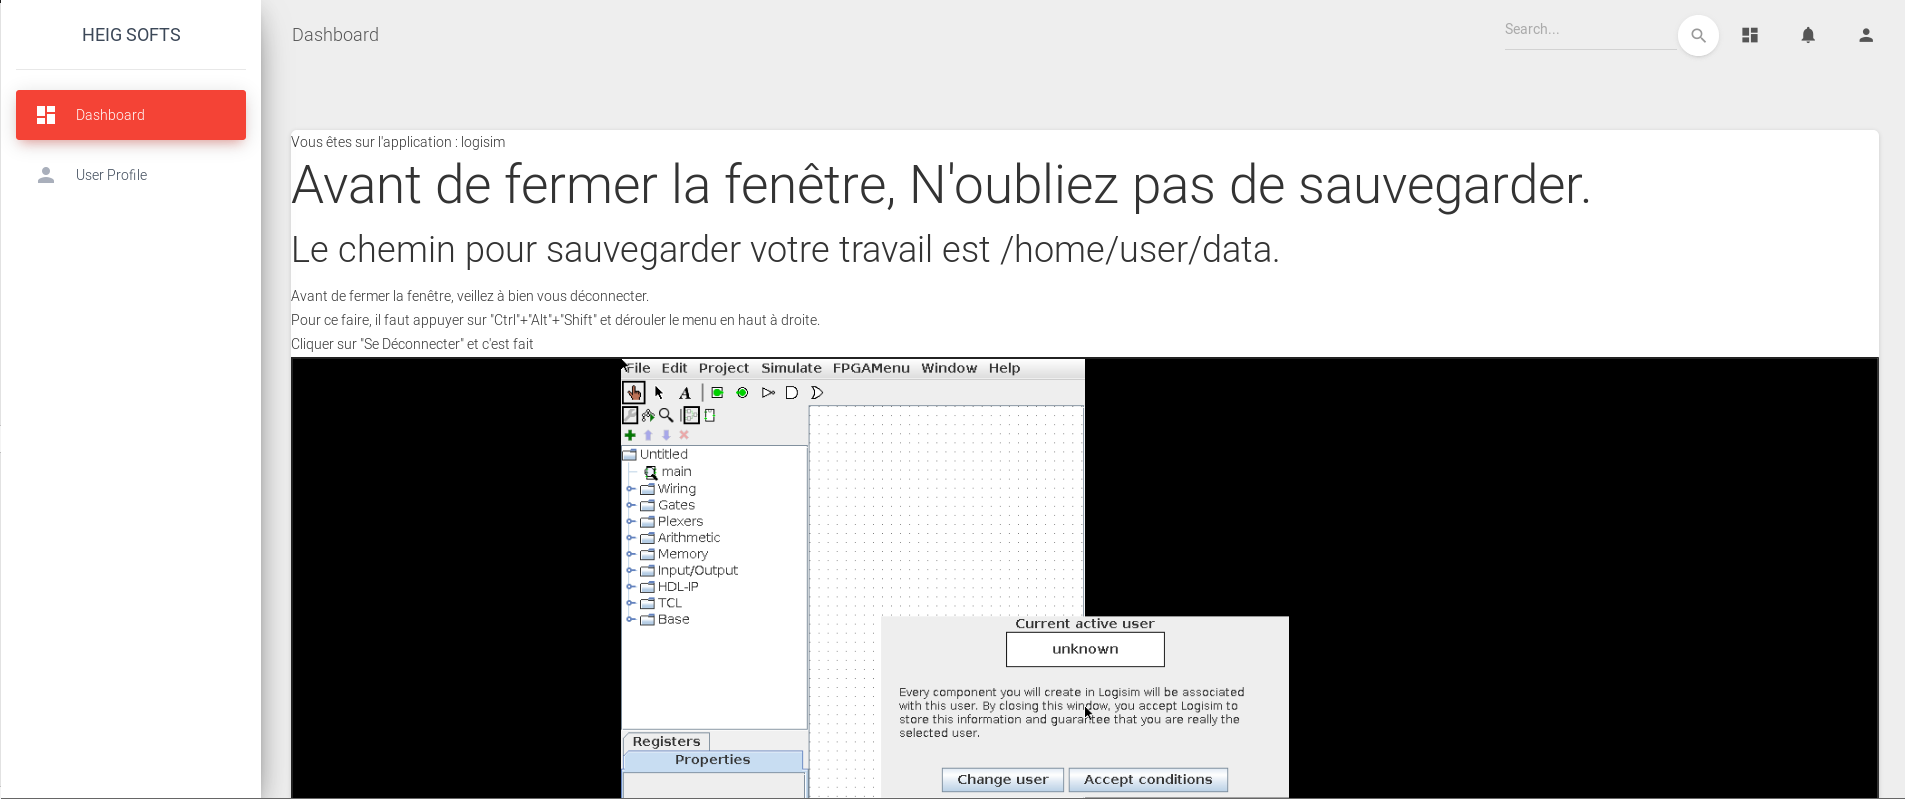
\includegraphics[scale=0.2]{images/website_logisim.png}
	\caption{Logisim}
	\label{fig:website_logisim}
\end{figure}
L'utilisateur peut donc modifier les fichiers présents dans le dossier partagé ou en rajouter s'il est administrateur.
La sauvegarde se fait dans tous les containers dans le dossier \com{/home/user/data}.
\newline
Pour avoir la fenêtre Guacamole sur l'interface, il est nécessaire de faire tourner deux services Web en parallèle.
Il faut configurer Tomcat de manière normale et avoir le client Guacamole sur le port 8080 du serveur.
En revanche, étant donné que ce travail a dû être fait sur une machine virtuelle,
afin de pouvoir avoir un rendu avec du \textit{PHP}, il faut faire tourner \textit{httpd} sur le port 81 et non 80 ou 8080.
Ensuite, à l'aide d'une iframe, il est possible d'appeler la page du client Guacamole avec dans l'url la paire "username:password" pour avoir un login automatique.
\newline
L'espace utilisateur sert simplement à montrer les informations de l'utilisateur connecté.
Il est envisageable d'ajouter une option pour les professeurs et administrateurs d'ajouter une application à un étudiant ou d'enlever à un étudiant, l'accès à une application.
Pour le moment, ce n'est pas encore implémenté.

\section{Tests}

\subsection{Serveur}
Les tests sur le serveur ont majoritairement porté sur la création des utilisateurs et le lancement du serveur \acrshort{vnc} avec les bons ports ouverts et le fichier de configuration guacamole écrit correctement.
Il a fallu tout d'abord lancé le script \com{main} et attendre la fin de son exécution. 
Le comportement attendu à la fin, avec la base de données actuelles, est : "trois utilisateurs avec leurs dossiers \com{/home} respectifs ont été créés".
Il faut aussi prendre en compte la population de ce dossier avec les répertoires contenant les fichiers de lancement des applications : \com{/home/<user>/<application>/launch.sh}.
\newline
Le script \com{main} finit son exécution sans encombre.
Une fois terminé, il est possible de voir les dossiers utilisateurs créés.
\begin{figure}[H]
	\centering
	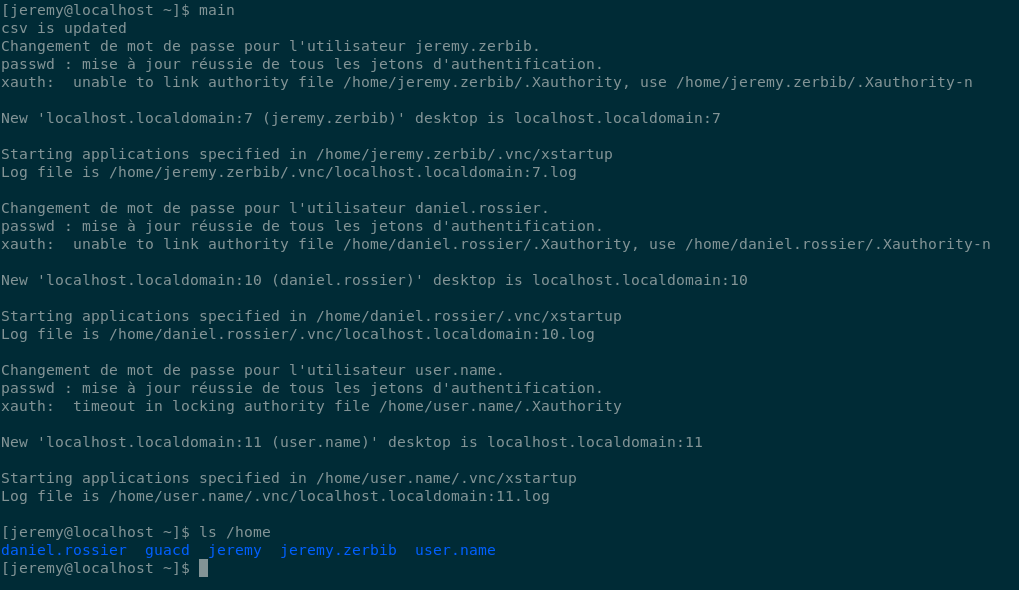
\includegraphics[scale=0.2]{images/main_home.png}
	\caption{Création des dossiers utilisateur}
	\label{fig:main_home}
\end{figure}



\subsection{Docker}

Une première phase de tests a été faite sur une machine utilisateur.
Cette phase consistait à tester le cloisonnement des applications avec l'ordinateur local.
Un volume partagé entre l'espace de \textit{test} et le container est créé permettant de rendre certains fichiers de configuration persistant et les travaux d'être sauvegardés.
Ce procédé est possible grâce à l'option suivante lors de l'appel à \com{docker run} : "\com{-v \${HOME}/logisim/data:/home/user/data}"
\newline 
Les tests ont donc consisté à lancer le container Mathematica et créer un nouveau fichier.
Il est possible de sauvegarder sur le filesystem du container le fichier créé mais il est impossible de le sauvegarder sur le filesystem de \textit{test}.
Après fermeture du container, aucun nouveau fichier n'est présent sur le \gls{filesystem} de \textit{test}.
Ce que cela implique est que si le fichier est sauvegardé  n'importe où à part le volume partagé, il est possible d'écrire en mémoire.
\newline 
Ensuite, un fichier est créé sur le volume partagé entre \textit{test} et le container en préambule de l'ouverture de ce dernier.
L'utilisateur a la possibilité de modifier le fichier et lors de la fermeture du container, il est possible de voir que le fichier modifié est présent dans le dossier.
\newline
Ensuite, il fallait vérifier que depuis le serveur, l'utilisateur puisse écrire sur un fichier donné et que suivant son rôle, il puisse ou non en créer un nouveau.
Dans tous les cas, il était impossible de créer un fichier depuis la plateforme Web.

\subsection{Guacamole}
Deux batteries de tests ont été faites sur Guacamole.
La première sur la page du client directement et la deuxième sur le site Internet afin de tester les interactions entre le servlet et la plateforme utilisateur.
\subsubsection{Client Guacamole}
Lors de l'arrivée sur la page du client Guacamole à l'adresse \com{localhost:8080/guacamole}, il est demandé de remplir un formulaire avec les identifiants d'un utilisateur.
Ces identifiants doivent figurer dans le fichier de configuration \com{user-mapping.xml}.
Il est à priori impossible de rentrer une paire "username/password" qui n'est pas dans ce fichier de configuration.
\newline
Avec la configuration du côte serveur \acrshort{vnc}, lors de la connexion sur Guacamole, il est possible de voir un terminal qui va lancer le container docker.
Un utilisateur pourrait être tenté de quitter l'application et accéder au terminal.
Guacamole gère ces interactions et lorsque l'utilisateur essaye de quitter l'application lancée de base, la connexion se coupe automatiquement.
Il est impossible d'accéder à une application qui n'est pas dans le fichier de lancement du serveur \acrshort{vnc}.
\newline
Ensuite, il a fallu vérifier que lorsque l'utilisateur quitte une session, cette dernière est bien supprimée.
Pour se déconnecter, il faut rentrer la combinaison "\textit{Ctrl + Alt + Shift}" et cliquer sur le menu déroulant en haut à droite du tiroir.
Ensuite, une fois déconnecter, il est impossible de se reconnecter sans rentrer les bons mots de passe.
\newline
En revanche, il est impossible de lancer deux utilisateurs sur la même fenêtre du même navigateur.
C'est à dire qu'il est impossible de lancer deux onglets en simultané avec deux utilisateurs différents.
Cela implique des complications pour la deuxième partie des tests.

\subsubsection{Site Internet et Guacamole}
A partir des tests effectués précédemment, il a été remarqué que si un utilisateur ne quitte pas explicitement pas une session sur Guacamole, il restera identifié tant que le navigateur n'est pas quitté ou la session terminée.
De ce fait, cela a posé des problèmes lors de certains tests effectués.
En effet, si l'utilisateur A se connecte sur son ordinateur et se déconnecte du site.
Il donne son ordinateur à l'utilisateur B et n'a pas fermé son navigateur entre temps.
Lorsque l'utilisateur B se connectera au site, il sera connecté sur la session Guacamole en tant que l'utilisateur A.
Pour le moment, aucune solution n'a été trouvée pour palier à ce problème.
C'est pour cela qu'un bandeau d'avertissement indique à l'utilisateur qu'il doit fermer sa session avec la marche à suivre pour faire ainsi.
Cela est dû au fait que le cookie de session créé lors de l'appel au client Guacamole via l'iframe ne peut pas se supprimer sur l'interface.
Les sessions ne sont pas les mêmes.
Il faudrait pouvoir envoyer un signal de déconnexion lors du logout du site.

\subsection{Site Internet}





\chapter{Conclusion}

\section{Point de situation au terme du rendu intermédiaire}
Jusqu'à lors, le travail a été uniquement théorique.
En effet, il a fallu effectuer des recherches et prévoir ce qui allait être fait dans la partie technique.
Des débuts de proof of concept ont été réalisés mais pas encore liés entre elles afin de fournir l'architecture souhaitée.
Du point de vue de la distribution, les scripts doivent être réalisés mais les librairies les composants ont été testées à différentes étapes de ce travail, ce qui rend la tâche un peu plus aisée.
Afin de mettre en avant le travail à effectuer, se référer à \ref{ch:final}.


% +---------------------------------------------------------------+
\cleardoublepage
\addcontentsline{toc}{chapter}{Bibliographie}
\bibliographystyle{plain}
\bibliography{chapters/biblio}
\nocite{*} %ajoute tout ce qu'il y a dans le bibtex

\listoffigures
\listoftables

% Annexes
% +---------------------------------------------------------------+
\appendix

\printglossaries

\chapter{Planning initial}
\label{ch:init}

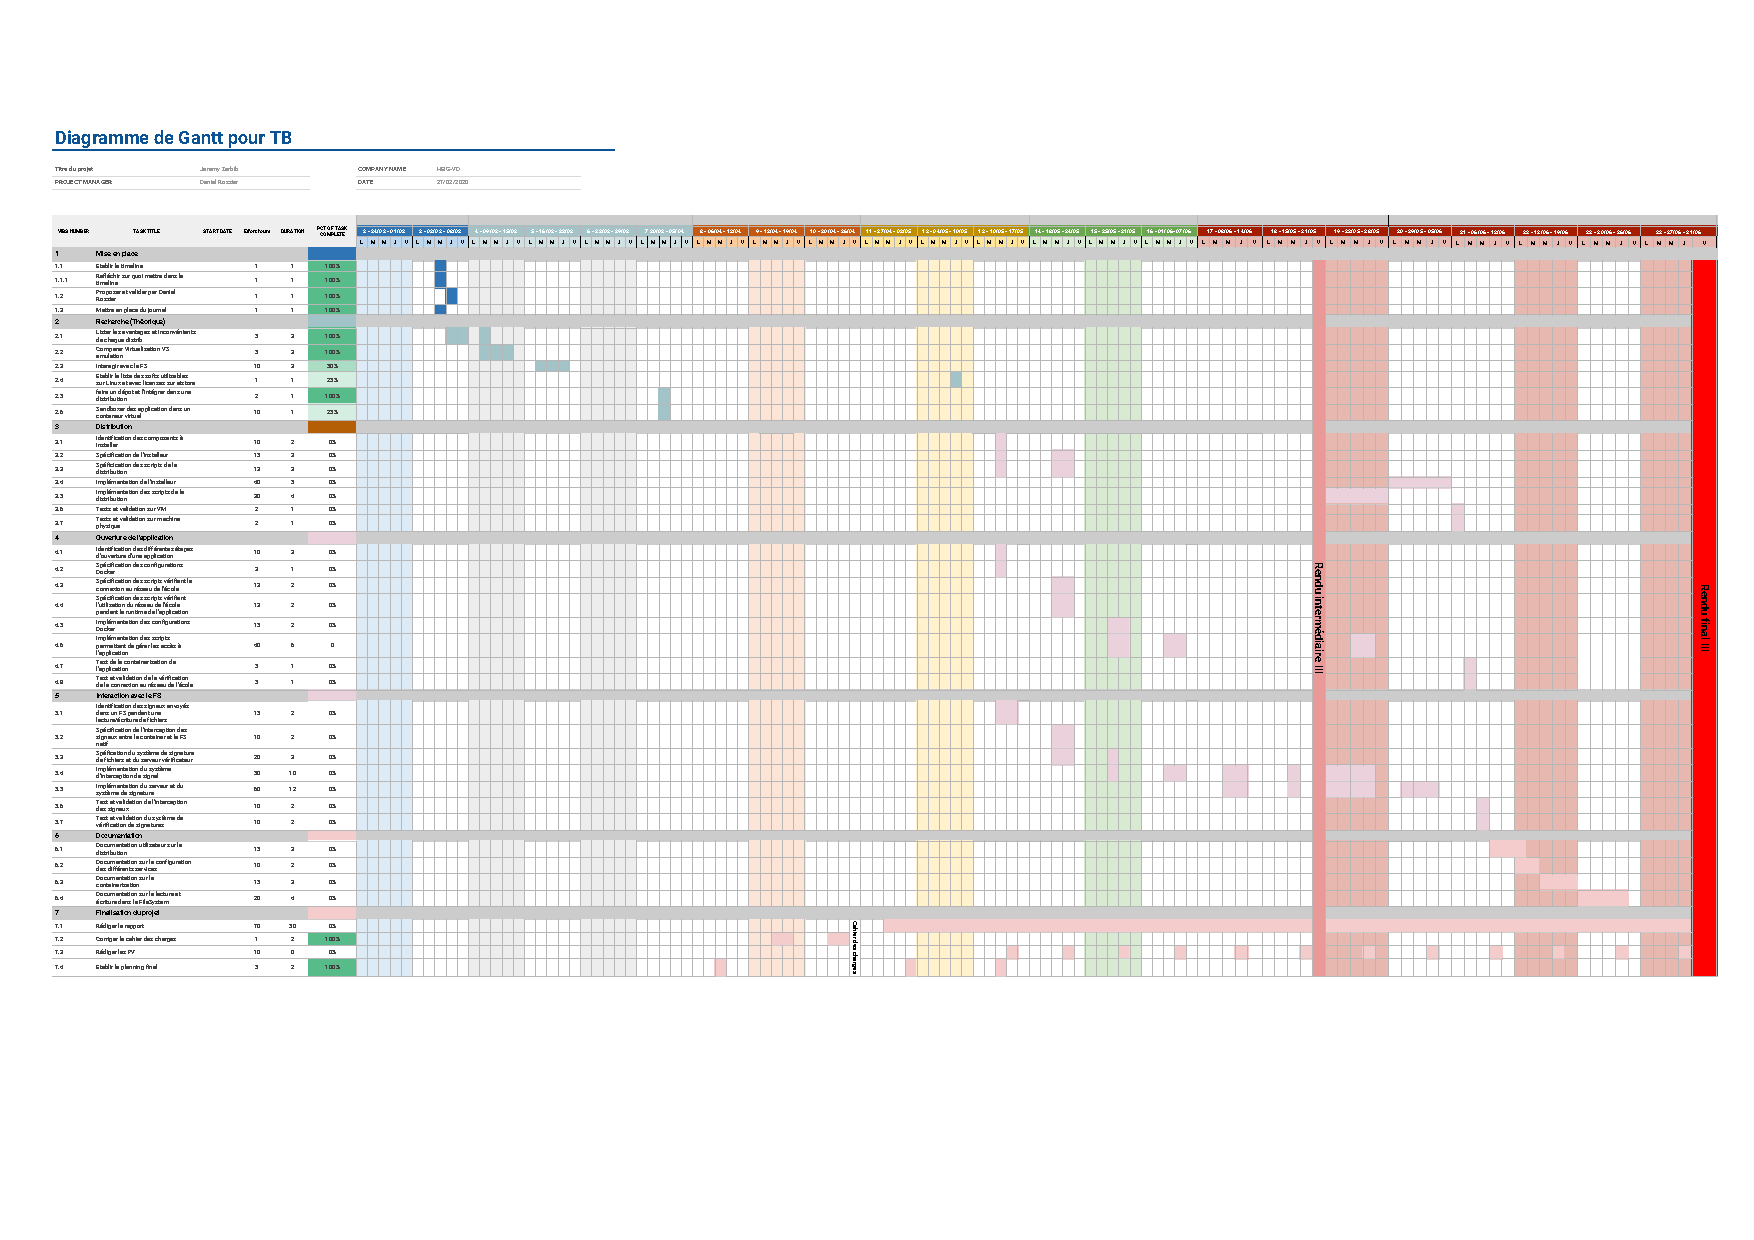
\includepdf[fitpaper,rotateoversize]{annexe/Timeline_projet.pdf}



\chapter{Planning final}
\label{ch:final}

Étant donné le changement de direction opéré, il a fallu corriger le planning.
La version présentée au préalable est valable en termes de délais mais des étapes ont changé.
Aussi, jusqu'en date du 19 juin, le planning reste valable.
Pour la suite du projet, en date du 19 juin 2020, un planning journalier sur deux semaines a été établi.
Il sera mis à jour et commenté de manière quotidienne afin de pouvoir affiner au maximum les différentes étapes journalière.
Aussi, une mise à jour hebdomadaire sera faite afin de garder deux semaines de planning effectif.
\newline

\begin{figure}[H]
	\centering
	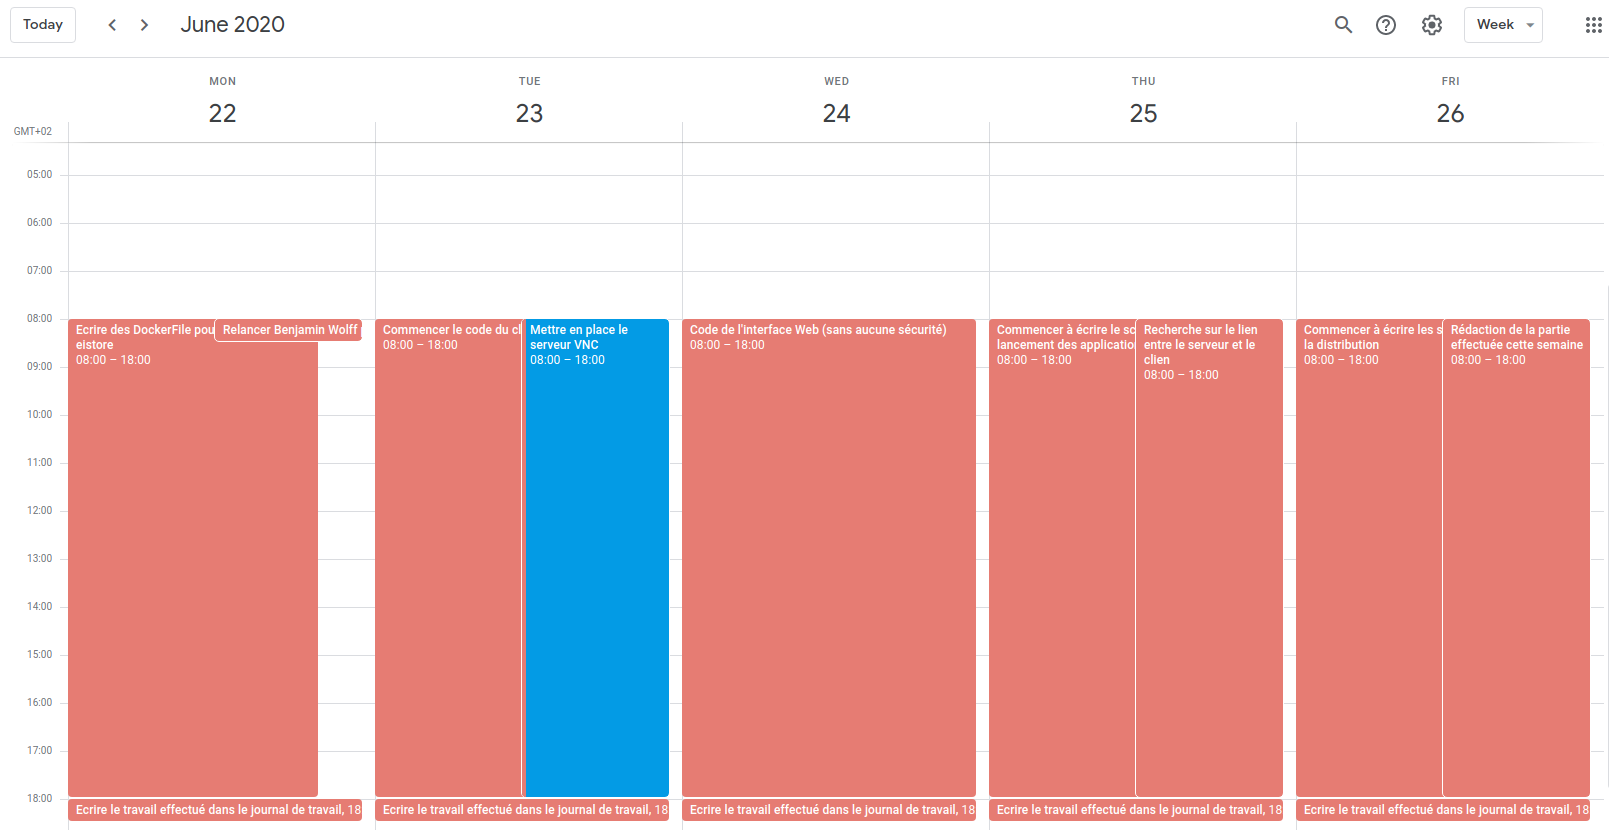
\includegraphics[scale=0.25]{images/planning/week1.png}
	\caption{Semaine 1 du travail à plein temps}
	\label{fig:week1}
\end{figure}


\begin{figure}[H]
	\centering
	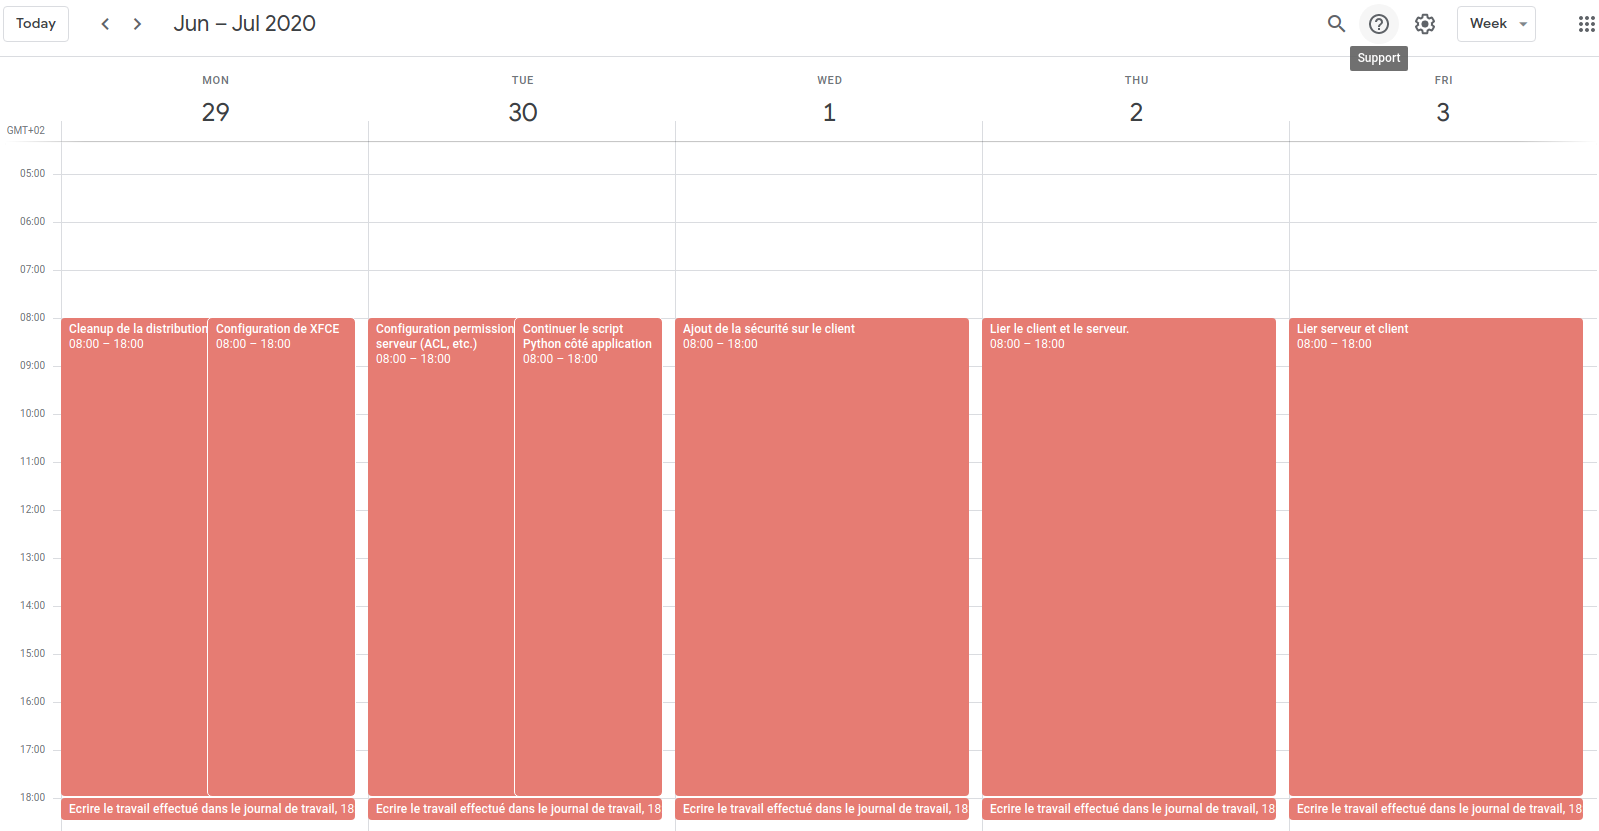
\includegraphics[scale=0.25]{images/planning/week2.png}
	\caption{Semaine 2 du travail à plein temps}
	\label{fig:week2}
\end{figure}


\begin{figure}[H]
	\centering
	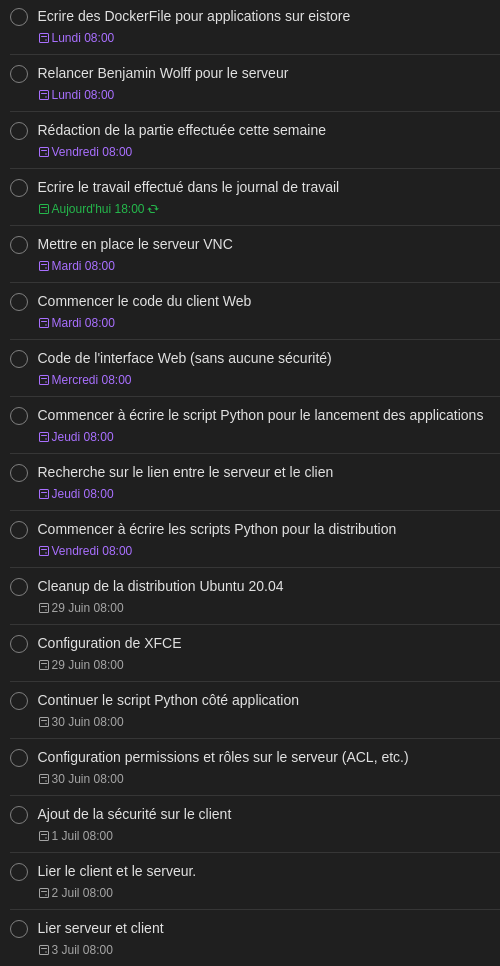
\includegraphics[scale=0.25]{images/planning/overview6Jul.png}
	\caption{Vue d'ensemble jusqu'au 6 juillet}
	\label{fig:ov6jul}
\end{figure}



\chapter{Documentation utilisateur}


\chapter{Outils utilisés pour la création et configuration de la distribution}


\chapter{Outils utilisés pour la gestion de licenses}


\chapter{Journal de travail}

\begin{landscape}

\begin{longtable}[c]{lp{10cm}rrrr}
    \caption{Journal de travail}\\

    \hline
    Date & Description & Rech. [h] & Dev. [h] & Rapport [h] & Admin [h] \\
    \hline
    \endfirsthead
    
    \hline
    Date & Description & Rech. [h] & Dev. [h] & Rapport [h] & Admin [h] \\
    \hline
    \endhead
    
    \multicolumn{6}{r}{\small \it Le journal de travail continue à la page suivante.} \\
    \normalsize
    \endfoot
    
    \hline
    \endlastfoot


  % Work
	25.02.2020 
	& Kick-off du projet et rdv avec M. Kapfer
	& 0 %recherche
	& 0 %dev
	& 0 %reporting
	& 2\\ %admin

	04.03.2020 
	& Travail sur le planning et mise en place du journal
	& 0 %recherche
	& 0 %dev
	& 0 %reporting
	& 4\\ %admin

	05.03.2020 
	& Recherche sur les différentes distributions et travail sur le planning
	& 2 %recherche
	& 0 %dev
	& 0 %reporting
	& 2\\ %admin

	06.03.2020 
	& Recherche sur les différentes distributions 
	& 3 %recherche
	& 0 %dev
	& 2 %reporting
	& 0\\ %admin

	10.03.2020 
	& Recherche sur les différentes distributions et début de la comparaison entre virtualisation et émulation
	& 3 %recherche
	& 0 %dev
	& 2 %reporting
	& 1\\ %admin
	
	
	11.03.2020 
	& Comparaison entre virtualisation et émulation
	& 5 %recherche
	& 0 %dev
	& 1 %reporting
	& 0\\ %admin
	
	12.03.2020 
	& Comparaison entre virtualisation et émulation
	& 2 %recherche
	& 0 %dev
	& 3 %reporting
	& 0\\ %admin
	
	17.03.2020 
	& Recherche sur les interactions dans un filesystem
	& 4 %recherche
	& 0 %dev
	& 0 %reporting
	& 0\\ %admin
	
	18.03.2020 
	& Recherche sur les interactions dans un filesystem
	& 5 %recherche
	& 0 %dev
	& 1 %reporting
	& 0\\ %admin
	
	19.03.2020 
	& Recherche sur les interactions dans un filesystem
	& 4 %recherche
	& 0 %dev
	& 2 %reporting
	& 0\\ %admin
	
	01.04.2020 
	& Création de dépôt et sandbox des applications avec GUI
	& 6 %recherche
	& 0 %dev
	& 2 %reporting
	& 0\\ %admin
	
	
	08.04.2020 
	& Recherche sur les interactions dans un filesystem
	& 4 %recherche
	& 0 %dev
	& 2 %reporting
	& 0\\ %admin
	
	09.04.2020 
	& Rédaction du cahier des charges
	& 0 %recherche
	& 0 %dev
	& 5 %reporting
	& 1\\ %admin
	
	10.04.2020 
	& Test des technologies de sandbbox avec Docker et rédaction du cahier des charges
	& 2 %recherche
	& 4 %dev
	& 3 %reporting
	& 1\\ %admin
	
	15.04.2020 
	& Test des technologies de sandbbox avec Docker
	& 2 %recherche
	& 4 %dev
	& 0 %reporting
	& 1\\ %admin
	
	16.04.2020
	& Fin de recherches sur les technologies Docker et QEMU et distribution.
	& 6 %recherche
	& 0 %dev
	& 1 %reporting
	& 1\\ %admin
	
	17.04.2020 
	& Setup du PC prêté par l'école
	& 0 %recherche
	& 6 %dev
	& 0 %reporting
	& 1\\ %admin
	
	22.04.2020
	& Setup du PC mais sans succès et finalisation du cahier des charges
	& 0 %recherche
	& 4 %dev
	& 3 %reporting
	& 1\\ %admin
	
	23.04.2020
	& Retour sur le cahier des charges et sur le planning.
	& 0 %recherche
	& 0 %dev
	& 4 %reporting
	& 2\\ %admin
	
	29.04.2020
	& Retour sur le planning et définitions de parties distinctes. Révision du planning par rapport aux heures de travail. Proof of concept des containers Docker avec GUI. Découverte de snap.
	& 3 %recherche
	& 4 %dev
	& 2 %reporting
	& 1\\ %admin
	
	30.04.2020
	& Recherche sur les interactions avec le filesystem.
	& 5 %recherche
	& 0 %dev
	& 2 %reporting
	& 1\\ %admin
	
	06.05.2020
	& Comparaison snap et Docker. Travail sur un nouveau PC car l'ancien de marchait pas -> il a fallu tout reconfigurer.
	& 5 %recherche
	& 0 %dev
	& 2 %reporting
	& 1\\ %admin
	
	07.05.2020
	& Retour sur le planning et modification complète des tâches à faire. Il a fallu remodeler avec l'approche \textbf{Recherches -> Spécifications -> Implémentations -> Validations}. Conclusion sur Snap vs Docker
	& 1 %recherche
	& 0 %dev
	& 4 %reporting
	& 2\\ %admin
	
	13.05.2020
	& Définitions de certains use-cases principaux. Correction du planning
	& 0 %recherche
	& 0 %dev
	& 6 %reporting
	& 0\\ %admin
	
	14.05.2020
	& Rendez-vous avec M. Kapfer qui a mené à un changement de vision sur le projet. Utilisation de la technologie VNC afin d'éviter les vérifications côté client. Retour sur le planning qui semble trop chargé.
	& 0 %recherche
	& 0 %dev
	& 2 %reporting
	& 2\\ %admin
	
	27.05.2020
	& Recherche sur la communication VNC et un client Web. Définition d'un use-case permettant de définir la sécurité et la robustesse d'une potentielle architecture.
	& 4 %recherche
	& 0 %dev
	& 2 %reporting
	& 1\\ %admin
	
	28.05.2020
	& Présentation du use-case. Définition des technologies à utiliser lors de cette phase. Définition d'un plan à suivre pour la suite du projet. Discussion avec M. Rossier sur le rapport intermédiaire et sur la suite du projet.
	& 0 %recherche
	& 0 %dev
	& 4 %reporting
	& 2\\ %admin
	
	03.06.2020
	& Création du canevas du rapport intermédiaire.
	& 0 %recherche
	& 0 %dev
	& 5 %reporting
	& 1\\ %admin
	
	04.06.2020
	& Discussion avec M. Rossier sur la structure et les changements à y apporter.
	& 0 %recherche
	& 0 %dev
	& 1 %reporting
	& 1\\ %admin
	
	15.06.2020
	& Rédaction du rapport intermédiaire.
	& 0 %recherche
	& 0 %dev
	& 6 %reporting
	& 1\\ %admin
	
	16.06.2020
	& Rédaction du rapport intermédiaire.
	& 0 %recherche
	& 0 %dev
	& 6 %reporting
	& 0\\ %admin
	
	17.06.2020
	& Rédaction du rapport intermédiaire.
	& 0 %recherche
	& 0 %dev
	& 7 %reporting
	& 0\\ %admin
	
	18.06.2020
	& Rédaction du rapport intermédiaire.
	& 0 %recherche
	& 0 %dev
	& 9 %reporting
	& 1\\ %admin
	
	19.06.2020
	& Rédaction du rapport intermédiaire.
	& 0 %recherche
	& 0 %dev
	& 6 %reporting
	& 0\\ %admin
	
	15.06.2020
	& Rédaction du rapport intermédiaire.
	& 0 %recherche
	& 0 %dev
	& 6 %reporting
	& 1\\ %admin
	
	22.06.2020
	& Création du Dockerfile pour Mathematica. Beaucoup de complexité sur cet outil, car l'installation se fait depuis un ISO. Il faut encore trouver le moyen de mettre en place un moyen de monter l'ISO. Pour le moment, l'installation marche mais pas encore connecté au XScreen et pas de volume pour la persistance.
	& 0 %recherche
	& 8 %dev
	& 0 %reporting
	& 0\\ %admin
	
	23.06.2020
	& Fin de la création du Dockerfile. Il reste à rajouter une persistance sur le container mais tout marche bien. Le GUI se lance et il est possible de travailler sur Mathematica et sauvegarder des fichiers sur le container. La création du volume permettra de pouvoir écrire sur le filesystem natif. Le SI fournira une VM CentOs, mais pas de date de fixée pour le moment donc prise de retard de ce côté. Du côté client, un template a été défini et sera travaillé demain. Un article a été écrit sur Discourse et d'autres seront rédigés au fur et à mesure de l'avancement du travail. Le serveur n'a pas pu être configuré car la personne qui s'en charge  aux SI n'a pas pu encore le faire. De plus, la version fournie de Mathematica n'était pas sous licence valable et un temps considérable a été perdu avant de trouver la cause. Le SI avait mis à disposition une version ultérieure à celle prise en charge ... 
	& 0 %recherche
	& 8 %dev
	& 0 %reporting
	& 1\\ %admin
	
	24.06.2020
	& Création du canvas du site. Les fonctionnalités principales sont énoncées et visibles mais aucune connexion au niveau du serveur. Le SI n'a toujours pas fait suite à la demande des specs de la VM...
	& 0 %recherche
	& 4 %dev
	& 0 %reporting
	& 1\\ %admin
	
	25.06.2020
	& Retour de M. Rossier sur le rapport intermédiaire. Le détail de ce retour se trouve dans le dossier de PV  à la même date qu'aujourd'hui. Note de 4 sur le rapport intermédiaire. Démonstration du travail effectué. Présentation du container Docker avec Mathematica et du Website sans aucun backend. Demande de M. Rossier de revoir le planning
	& 0 %recherche
	& 0 %dev
	& 0 %reporting
	& 1\\ %admin
	
	26.06.2020
	& Refonte du planning et documentation de la containerisation.
	& 0 %recherche
	& 0 %dev
	& 4 %reporting
	& 2\\ %admin
	
	29.06.2020
	& Configuration de l'environnement Ubuntu pour la distribution. Suppression de beaucoup de bloatwares, il en reste encore. Écriture du script permettant de configurer les différents services de l'école. Après réunion avec GAPS, le bot ne sera pas utilisé pour le moment, une deuxième aura lieu dans quelques temps. Écriture d'un script de dépendances à enlever et à rajouter pour la suite.
	& 1 %recherche
	& 4 %dev
	& 1 %reporting
	& 1\\ %admin
	
	30.06.2020
	& Création du Dockerfile pour Logisim. Il existe une particularité sur ce container par l'utilisation de Java. Il faut rajouter \com{docker} à l'environnement graphique \com{xhost} manuellement. Après réunion avec M. Rossier, il a fallu refaire le planning et j'ai eu un feedback plus complet sur le rapport intermédiaire.
	& 1 %recherche
	& 5 %dev
	& 1 %reporting
	& 1\\ %admin
	
	01.07.2020
	& Travail à 100\% sur le script permettant de se connecter sur les différents services de l'école. Réussite de connexion au réseau HEIG-VD et eduroam. Création de la connexion VPN.
	& 1 %recherche
	& 4 %dev
	& 1 %reporting
	& 1\\ %admin
	
	02.07.2020
	& Finir le script permettant de centraliser. Discussion avec Alexandre Duc pour m'éclairer sur le stockage de credentials. Il faut plutôt utiliser le keyring de Ubuntu et pas refaire une sécu dessus. L'utilisation de LDAPs est suffisante dans le cadre pratique. En théorie, il faut éviter -> à documenter. La documentation pour eduroam est fausse au SI. Il faut aller sur le site de eduroam (officiel) et prendre le script d'installation de eduroam. Pour le moment, le réseau a été configuré sur le modèle de l'école mais il faut changer ça 
	& 2 %recherche
	& 5 %dev
	& 1 %reporting
	& 1\\ %admin
	
	03.07.2020
	& Rédaction du travail de la semaine
	& 2 %recherche
	& 0 %dev
	& 5 %reporting
	& 0\\ %admin
	
	06.07.2020
	& Finalisation du script de centralisation. Ajout de certaines conditions et modularisation du script- J'ai essayé de configurer un rendu graphique avec le serveur fourni par l'école, avec l'aide de David Truan, mais impossible. Le GUI ne se charge pas via \com{ssh}, ni via VNC. Du coup, j'ai pris la décision de travailler sur une VM. Afin de pouvoir avancer dans mon travail, on simulera un serveur avec une VM. Du côté distribution, j'ai essayé de générer un ISO mais pas encore réussi. Je continuerais ce travail plus tard.
	& 2 %recherche
	& 4 %dev
	& 1 %reporting
	& 0\\ %admin
	
	07.07.2020
	& Démonstration du script le matin à Daniel Rossier et explication de la situation. Essai de VNC sur VM, mais CentOs bloque trop de paramètres Docker et VNC. J'ai donc essayé de configurer quelque chose de performant mais aucun résultat.
	& 3.5 %recherche
	& 3.5 %dev
	& 1 %reporting
	& 0\\ %admin
	
	07.07.2020
	& J'ai donc essayé différentes distribs afin de trouver la plus adéquate à cette tâche. A priori, Manjaro, basé sur Arch, serait le choix que je vais faire. En effet, il y a toujours moyen de mettre en place un système d'ACL et Docker marche correctement. Ubuntu Server ne permet pas de mettre en place facilement les ACL ou le VNC. Manjaro permet de faire le tout sans trop de soucis à priori. 
	& 2 %recherche
	& 5 %dev
	& 1 %reporting
	& 0\\ %admin
	
	08.07.2020
	& J'ai réussi à mettre en place un serveur VNC et le lire avec le client VNC sur un ordinateur. Reste maintenant à comprendre comment mettre en place ça sur un site Internet. La technologie que j'avais trouvé ne permet pas de créer des interactions avec l'ordinateur diffusé. Il existe un "framework" qui permet de diffuser des flux sur un site Internet "Apache Guacamole". Cette technologie est à étudier mais permet de faire en sorte qu'un utilisateur peut interagir avec un ordinateur distant.
	& 6 %recherche
	& 2 %dev
	& 1 %reporting
	& 0\\ %admin
	
	09.07.2020
	& Apprentissage de Guacamole afin de mettre en place une connexion VNC avec des interactions sur l'ordinateur diffusé.
	& 5 %recherche
	& 4 %dev
	& 1 %reporting
	& 0\\ %admin
	
	10.07.2020
	& Ecriture du travail de la semaine 
	& 0 %recherche
	& 0 %dev
	& 6 %reporting
	& 0\\ %admin
	
	13.07.2020
	& Setup du serveur avec une base de données. La base de données renferme toutes les informations des utilisateurs de l'école. Il faut encore tester la robustesse du script avec quelques milliers de données mais le comportement global du script est le suivant : Récupération des données avec une requête SQL -> Parsing des données afin de créer un userspace pour chaque nouvel utilisateur, affectation à un groupe selon le rôle et création des dossiers pour chaque application. Chaque application est construite de base et depuis le site, un script sera appelé et lancera le container.
	& 2 %recherche
	& 6 %dev
	& 1 %reporting
	& 0\\ %admin
	
	14.07.2020
	& Test du script. Cleanup et optimisation au maximum pour le moment. Il reste encore quelques tests et c'est tout bon. Début de setup du serveur Guacamole. Pas mal de complications et ça ne marche toujours pas.
	& 3 %recherche
	& 5 %dev
	& 1 %reporting
	& 0\\ %admin
	
	15.07.2020
	& Setup continué de guacamole et j'ai réussi à le déployer. Le soucis reste la connexion VNC. En local, avec un VNCViewer, ça marche sans problème mais pas sur Guacamole
	& 0 %recherche
	& 0 %dev
	& 6 %reporting
	& 0\\ %admin
	
	16.07.2020
	& Contact de Loic Haas pour lui demander de l'aide sur Guacamole. Du coup en l'attendant, j'ai travaillé un peu sur le rapport. J'ai commencé les corrections par rapport au rendu intermédiaire afin de pouvoir partir sur une bonne base pour le rapport final. Après discussion, il a été possible de lancer et de faire tourner le framework.
	& 3 %recherche
	& 3 %dev
	& 3 %reporting
	& 0\\ %admin
	
	16.07.2020
	& Rédaction du rapport
	& 0 %recherche
	& 0 %dev
	& 6 %reporting
	& 0\\ %admin
	
\end{longtable}


\end{landscape}


\end{document}
